% !TEX root = ../../book.tex
\chapter{Trading Fundamentals \label{chap:ch_trading_fund}}


%%%%%%%%%%%%%%%%%%%%%%%%%
%%%%%%%%%%%%%%%%%%%%%%%%%
\begin{comment}
\section{Max old stuffs temporary reinstated for my ease of use...}


% Algorithmic Trading: Some Basic Elements
\subsection{Algorithmic Trading: Some Basic Elements}

As such, algorithmic trading can be described as a broader field combining several areas such as mathematical modeling, computer science and statistical analysis. Quantitative strategies, such as the ones detailed in the subsequent chapters, call for robust and methodical research, a good understanding of economics fundamentals, while the amount of data available and the complexity of reproducing realistic trading conditions require a reliable and fast infrastructure for backtesting and calibrating models.


More simply, the practitioner working on developing quantitative algorithmic strategies goes through the following steps:

\begin{itemize}
\item \textbf{Data collection:} As mentioned previously, there is no dearth of available data. That said, the researcher needs to put particular emphasis on understanding the data structure as well as the methodology used to collect it (Which data feed is used? At what point is the data time stamped? What is the impact on recording the market performance of when there are activity bursts? How to order in the correct sequence, data coming from different origins or different asset classes in the correct time scale? etc.). High frequency data tends to be noisy, and one of the significant challenges faced in practice is to devise appropriate mechanisms to clean-up possibly corrupted data, to handle missing data, to tag outliers so that they can be isolated from the general modeling and to study how to use them for modeling extreme scenarios that may arise in the future. Failure to properly correct for errors in the data inevitably will lead to misspecified trading strategies that will not perform as expected.


\item \textbf{Modeling:} The core of the subsequent chapters will cover in detail the models commonly used in existing quantitative strategies. These models cover the diverse nature of the trading data.  Particular attention should be paid to the underlying assumptions of the model (characteristics of the distribution, independence, stationarity, etc.), as well as the robustness and stability of the calibration under model deviations. While violation of model assumptions is one of the most common pitfalls encountered in practice, model misspecification (whether due to missing variables or inclusion of wrong variables) can also lead to significant bias (see Rao (1973)~\cite{rao1973}). 


\item \textbf{Backtesting:} Once the strategy is designed, the next step involves backtesting it, both on in and out of sample data. The objective is to determine the behavior and profitability of the strategy over time in order to fine tune the calibrated parameters. Backtesting can be carried out with different objectives, from simply maximizing returns to maximizing risk-adjusted returns metrics such as Sharpe ratio or Sortino ratio. However, a key factor in successful and realistic backtesting depends on the assumptions of the model. Among the relevant issues to consider for execution: the fill probability (for passive orders), the models for market impact that determines the actual transactions and the scalability of the strategy all require particular attention. Additionally, for high frequency strategies, the backtesting should account for bursts of market events and latency effects. Finally, while the goal of backtesting is to find the optimal model, the most common pitfall encountered by practitioners is overfitting with a large set of parameters that simply introduce noise rather than capturing the signal (see Easley, Lopez de Prado and O'Hara (2014)~\cite{easley}).  


\item \textbf{Execution:} The final step involves deploying the strategy in production and continually monitoring its performance to determine if there is a need for potential adjustments. The field of Transaction Cost Analysis is relevant to both developers of algorithmic trading strategies and users of strategies developed by third parties such as sell-side brokers. We give some initial thoughts on this topic in the remainder of the chapter.
\end{itemize}


\end{comment}
%%%%%%%%%%%%%%%%%%%%
%%%%%%%%%%%%%%%%%%%%



\section{A Brief History of Stock Trading}

\noindent\textbf{Why Do We Trade:} Companies need capital to run and expand their businesses. To raise capital, they can either borrow money, paying it back over time with interest, or they can sell a stake (equity) in the company to an investor. As part owner of the company the investor would then receive a portion of the profits in the form of dividends. Equity and Debt, being scarce resources, have also intrinsic values that change over time; their prices are influenced by factors related to the performance of the company, existing market conditions and, in particular, the future outlook of the company, the sector and the economy as a whole. For instance, if interest rates charged to borrow capital change, this would affect the value of existing debt since its returns would be compared to the returns of similar products/companies that offer higher/lower rates of return. When we discuss trading in this book we refer to the act of buying and selling debt or equity (as well as other types of instruments) of various companies and institutions among investors who have different views of their intrinsic value.


These secondary markets transaction also serve a purposes of price discovery (O'Hara (2003)~\cite{ohara}). Buyers and sellers meet and agree on a price to exchange a security. When that transaction is made public it, in turn, informs other potential buyers and sellers of the most recent valuation of the security.  


How the trading process has evolved over the last 200 years makes for an incredible tale of ingenuity, fierce competition and adept technology. To a large extent It was (and continues to be) driven by the positive (and at times not so positive) forces of money and greed, creating over time, a highly complex but, in most cases, amazingly efficient mechanism for evaluating the real value of a company. \\


\noindent\textbf{The Origins of Equity Trading:} The tale begins on May 17, 1792 when a group of 24 brokers signed the Buttonwood Agreement which bound the brokers to trade only with each other under specific rules. This agreement marked the birth of the New York Stock Exchange or NYSE. While the NYSE is not the oldest Stock Exchange in the world,\footnote{this honor sits with the Amsterdam Stock Exchange dating back to 1602} nor the oldest in the US \footnote{the Philadelphia Stock Exchange has a 2 year head start having been established in 1790} it is without a question the most historically important one and the undisputed symbol of financial markets. Thus it is, in our opinion, the most suitable place to start off our journey. The NYSE soon moved their operations to the nearby Tontine Coffee House and subsequently to various other locations around the Wall Street area before settling in the current location on the corner of Wall St. and Broad St. in 1865.


For the next almost 200 years, stock exchanges evolved in complexity and in scope but remaining conceptually unchanged, functioning as a physical locations where traders and stockbrokers met in person to buy and sell securities. Most of the exchanges settled to an interaction system called Open Outcry where new orders were communicated to the floor via hand signals and with a Market Maker facilitating the transactions often stepping in to provide short term liquidity. The advent of the telegraph and subsequently the telephone had dramatic effects in accelerating the process and the dissemination of the information but not on the fundamental process through which trading was done.\\


\noindent\textbf{Electronification and the Start of Fragmentation:} This all changed in the late 60s and early 70s. In 1971, the NASDAQ Stock Exchange launched as a completely electronic system. Initially started as a quotation site, it turned into a full exchange and  quickly became the second largest US exchange by market capitalization. In the meantime, another trend had already started. In 1969, the Institutional Networks Corporation launched Instinet, a computerized link between banks, mutual fund companies, insurance companies so that they could trade with each other with immediacy, completely bypassing the NYSE. Instinet was the first example of an Electronic Communication Networks (ECNs), an alternative approach to trading that grew in popularity in the 80s and 90s to include other notable venues like Archipelago and Island ECNs.


This evolution started a trend in market structure that only got more accentuated over time resulting in ``liquidity fragmentation'' meaning that all available interest for a security is not centralized but rather distributed across multiple ``liquidity pools.''  This decentralization of liquidity created significant challenges to the traditional approach of trading and accelerated the drive toward electronification.\\


\noindent\textbf{The Birth of HFT and Algorithmic Trading:} The year 2001 brought another momentous change in the structure of the market. On April 9, 2001, the SEC mandated that the minimum price increment on any exchange should change from 1/16th of a dollar ($\approx6.25$ cents) to 1~cent.\footnote{ The 1/16th price increment was a vestige of Spanish monetary standards of the 1600s when dobloons where divided in 2, 4, 8 parts} This seemingly minor rule change with the benign name of `Decimalization' (moving from fractions to decimal increments) had a dramatic effect, causing the average spread to significantly drop and with that, the profits of market makers and broker dealers. The reduction in profit forced many market making firms to exit the business and thus, reduced the  available market liquidity. To bring this liquidity back, exchanges introduced the maker-taker fee model which would compensate, in the form of rebates, the trader that provided liquidity (makers) while charging the regular fee to the consumer of liquidity (takers).\footnote{For some readers the concepts of providing and taking liquidity might be murky at best. No fret, this will all become clear when we discuss the trading process and introduce market microstructure}


This decision created unintended consequences. In this new setup if one could provide liquidity while limiting liquidity taking, one could make a small profit, due to the rebate with minimal risk and capital. This process would need to be fairly automated as the per trade profit would be minimal and requires to trade a lot to generate real revenue. It would also need to be fast because position in the order book and speed of cancellation of orders are both critical for profitability. This led to the explosion of what today we call High Frequency Trading (HFT) and to the wild technology arms race to become faster and faster that has swept the industry in the last 15 years. HFT style trading (what used to be called opportunistic market making) already existed but never as a significant portion of the market. At its peak it was estimated that more than 60\% of all trading was generated by HFTs.


With trading costs decreasing trading volume increased but the drop in trading commission and profitability forced broker dealers to start automating some of their more mundane trading activities. Simple workflow strategies slowly evolved into a field that we now call Algorithmic Execution which is one of the main topic of this book. \\

\noindent\textbf{Dark Pools and Reg NMS:} Over the years, fragmentation has continued to increase and the changes in market structure evolved further. New venues have surfaced with different value propositions: allow traders to find a block of liquidity without necessarily conveying that information to a block trader or market maker thus reducing risk of information leakage. No market data is published from these venues, only the notification of a trade after the fact is conveyed; these venues are aptly, but somewhat ominously, named Dark Pools.


In 2005, Regulation National Market System (Reg NMS) was introduced to try to protect investors from the increase in trading complexity and fragmentation, and further accelerated the transformation of market structure in the US\footnote{equivalent regulation had a similar impact in Europe - see MiFID}. Through its two main rules, the Reg NMS intent was to promote best price execution for investors by encouraging competition among individual exchanges and individual orders. The Access Rule promoted non-discriminary access to quotes displayed by Self-Regulatory Organization (SRO) trading centers as well as established a cap, limiting the fees that a trading center can charge for accessing a displayed quote. The Order Protection Rule required trading centers to obtain the best possible price for investors when such price was represented by an automated immediately accessible quote. In essence, aside from a series of exemptions, the Order Protection Rule mandated market participants to transact first at a price better or equal to the National Best Bid Offer (NBBO).


The latter rule, in particular, had a significant effect on the US market structure. Market makers, who had traditionally been competing for quotes on a given exchange, quickly became multi-venue market makers by leveraging technology to process real time  quotes from all Reg NMS protected venues to determine where and at what price to provide their own quotations. Automated market makers therefore played a critical role in linking various trading venues and allowing for fragmentation to increase. The NYSE market share in NYSE-listed stocks was still above 80\% in 2005 but that number quickly declined as Reg NMS facilitated competition among venues to reduce NYSE's share to 25\% by 2010. 


As fragmentation increased, speed and technology became major differentiating factors of success for market makers and other participants. The ability to process market data, analyze it, and submit one's orders faster than competing participants meant capturing fleeting opportunities or successfully avoiding adverse selection. To gain or maintain an edge, market participants heavily invested in technology, faster networks, and installed their servers in the same data centers as the venues they transacted on (co-location). \\


\noindent\textbf{Conclusion:} This brings us to present times. This whirlwind tour was not intending to be comprehensive but simply to provide the background forces and dynamics that led to the dizzying complexity of modern market structure which would seem hard to comprehend without the appropriate context. Readers might be wondering why this treatment of the history of trading was limited to the US alone. This is not meant to imply that the rest of the world stayed still. Europe and Asia had somewhat slower and somewhat compressed evolution. The main features are more or less similar but have had a much less colorful and exciting evolution. 



% Market Structure and Trading Venues: A Review
\section{Market Structure and Trading Venues: A Review}

% Equity Markets Participants
\subsection{Equity Markets Participants} 

With the context acquired in the previous section, we can now jump in a few brief review on the state of modern Market Structure. In order to get a sense of the underpinning of Equity markets, it is important to understand the the various participants, why they trade and what their principal focus is. \\


\noindent\textbf{Long Only Asset Managers:} These are the traditional Mutual Funds providers like Vanguard, Fidelity, etc. A meaningful portion of the US families regularly invests in mutual funds for their retirement as part of their company's pensions funds, 401ks, and other retirement instruments and many of the largest providers have trillions of dollars under their management. They are called Long Only because they are restricted from short selling (where you borrow shares to sell in the market in order to benefit from a price drop) and can only profit through dividends and price appreciation. These firms need to continuously trade in order to re-balance their large portfolios to manage in-flows, out-flows, and to achieve the fund's objective which is to track and hopefully beat a competitive benchmark. The time horizon these investors care about is in general long, from months to years. Historically less sophisticated in their trading operations the participant have been less concerned with transaction costs since the investment time scales are long and the returns they target dwarf the few dozen basis points incurred in transaction costs. What they are particularly concerned about is information leakage, that  other participants in the market  (in particular HFTs) realize what they are up to and profit from the information to the detriment of the fund's investors. \\


\noindent\textbf{Long-Short Asset Managers and Hedge Funds:} There are a myriad of large and small firms catering to institutional clients and wealthy investors. They often run multiple strategies, most often market-neutral long-short strategies, holding long and short positions in order to have reduced market exposure and  thus hopefully perform well in both raising and falling markets. Investors of this type include firms like Bridgewater, Renaissance Technologies, Point~72 (former SAC Capital), and many others. Their time horizon is as long as the strategies they employ, but in general they are shorter than their Long Only counterparts. They also tend to be more sophisticated traders who are really careful to minimize transaction cost since they often make many more smaller bets and the transaction costs can be a significant fraction of their expected profits. \\


\noindent\textbf{Broker-Dealers (aka Sell Side):} They sit in between the ``Buy Side'' (generic term for asset management firms and hedge funds) and the various exchanges.\footnote{Note that only member firms are allowed to trade on exchange and most asset management firms are non-members} They can act either as Agent for the client (i.e. Broker) or provide liquidity as Principal (i.e. Dealer) from their own accounts. They historically had  also large proprietary trading desks investing the firm's capital using strategies not dissimilar to the ones Hedge Funds use. Since the introduction of the Dodd-Frank Act\footnote{\url{https://en.wikipedia.org/wiki/Dodd\%E2\%80\%93Frank_Wall_Street_Reform_and_Consumer_Protection_Act}} the amount of proprietary risk that a firm can carry has dramatically decreased and most banks shed large part of their proprietary trading activities either shutting down the desks or spinning them off in independent hedge funds. \\


\noindent\textbf{HFTs and ELPs (Electronic Liquidity Providers), DMMs (Designated Market Makers):} These participants generate returns by acting as facilitators between the above participants, providing liquidity and then unwinding it at a profit. They can also be aggregators of retail liquidity, e.g. individual investors trading using online providers like ETrade. Likely the most technology savvy operators in the market place, they leverage ultra-low-latency infrastructure to be extremely nimble in getting in and out of positions and taking advantage of tiny mis-pricing. 


%  Equity Markets Watering Holes
\subsection{Equity Markets Watering Holes}

Now that we know who the players are, we briefly review various approaches they use to access liquidity. \\


\noindent\textbf{Exchanges:} This is the default approach to trading and still accounts for about 60--70\% of all activity. This is where an investor will go for immediacy and for a more certain outcome. Because the full order-book of an exchange is public and arrivals/cancellations are all published, the trader knows almost exactly what liquidity is available and can plan accordingly. This, unfortunately, comes at a cost as the same information is known by all other participants especially (due to their often technological advantages) the ones whose strategies are looking for patterns of large directional trades. A trader that needs to buy or sell in size will need to be very careful on how much information their trades disseminate; otherwise, that trader may pay dearly. The whole field of Algorithmic Execution evolved as an effort to trade large sizes while minimizing market impact and information leakage. \\


Apart from leakage concerns interacting with exchanges is arguably the most basic approach to trading. At the time of this writing, a US equity trader can buy or sell stocks in 14 registered exchanges.\footnote{\url{https://www.sec.gov/fast-answers/divisionsmarketregmrexchangesshtml.html}} As mentioned before with RegNMS, these exchanges are all ``protected'' meaning that liquidity at the best price cannot be ignored, and an exchange will need to reroute to other exchanges where price is better (charging a fee for the honor). This creates a lot of complexity and is solved via technology and automation through the use of Smart Order Router.


Recent years have seen a consolidation of these exchanges in the hands of three main players: NYSE, NASDAQ and CBOE/BATS. Here is a list of venue operated by each:
        \begin{itemize}
        \item NYSE: NYSE, Arca, MKT LLC ( former AMX, American Stock Exchange), NSX (form National Stock Exchange), CHX (former Chicago Stock Exchange)
        \item NASDAQ:  NASDAQ, PHLX (former Philadelphia Stock Exchange), MRX (former ISE Mercury), ISE (former International Securities Exchange), GEMX (former ISE Gemini), BX (former Boston Stock Exchange)
        \item CBOE/BATS: CBOE, BZX (former BATS), BYX (former BATS-Y), EDGA, EDGX, C2
        \end{itemize}
As a notable mention, the newest exchange and as of now the only independent exchange, is The Investors Exchange or IEX which we will discuss further in this section.


An interesting observation is that this consolidation was not happened with a contemporaneous reduction in fragmentation. These venues continue to operate as separate pools of liquidity. While the exchange provider make valid arguments that these exchange provide different business proposition there is a growing concern across the industry that the revenue model for these exchanges is now largely centered around market data and exchange connectivity fees. Because the venue quotes are protected, any serious operator will need to connect with this exchanges and leverage their direct market data feeds in their trading applications and with more exchanges the more connections and fees these exchange can charge. Recently regulators are starting to weigh in on this highly contentious topic.\footnote{\url{https://www.sec.gov/news/public-statement/statement-chairman-clayton-2018-10-16}}


It is also interesting to note that these exchanges are almost all hosted in one of four data centers located in the New Jersey countryside: Mahwah, Secaucus, Carteret, Weehawken. The distance between these data centers adds some latency in the dissemination of information across exchanges creating latency arbitrage opportunities as super fast HFTs co-locate in each data center and leverage the best available technology such as microwave towers. They can see market data changes before others do and either trade ahead or cancel their own quotes to avoid adverse selection (a phenomenon known as liquidity fading).


All exchanges have almost exactly the same trading mechanism and from the trading perspective behave exactly the same way during the continuous part of the trading day (i.e excluding the opening and closing auctions which we will discuss in a separate section). They provide visible (meaning that market data is disseminated) order books and operate in a price/time priority basis. Most of them use the Maker-Taker fee model that we discussed earlier but a few: BYX, EDGA, NSX, have adopted an `Inverted' fee model where posting liquidity incurs a fee while a rebate is provided for taking liquidity. This subtle but significant difference causes these venues to display a markedly different behavior. The cost for providing liquidity removes the incentive of rebate seeking HFTs; however because the taker is compensated, these venues are used first when needing urgent liquidity. This in turn brings in passive liquidity providers who agree to pay for trading passively at that price. This interplay creates subtle and still not well understood dynamics about how the market as a whole behaves.


Finally, some observations about IEX. It started as an ATS whose main innovation is a 38-mile coil of optical fiber placed in front of its trading engine. This introduces a 350 microseconds delay each way aptly named a ``speed bump'' that is meant to remove the speed advantages of HFTs. The intent is to reduce the efficacy of the more predatory tactics and thus provide a liquidity pool that is less ``toxic''. On June 17, 2016 IEX became a full fledged exchange after a very controversial process, and marketed themselves as an exchange that would be different and would attract substantial liquidity due to its innovative speed bump. As of 2018, this potential remains still somewhat unrealized and IEX has not moved much from the 2\% market share of which 80\% is still in the form of hidden liquidity. That being said IEX has established itself as a vocal critic of the current state of affairs continuing to shed light to some of the potential conflicts of interests that have arisen. At the time of this writing IEX does not charge any market data fees.\footnote{\url{https://iextrading.com/trading/market-data/}} \\


\noindent\textbf{Alternative Trading Systems/Dark Pools:} As discussed above trading in large blocks in exchanges is not a simple matter and requires advanced algorithms and smart order routers. Even then the risk and realized costs due to information leakage can be significant. Dark Pools were invented to counterbalance this situation. One investor can have a large order ``sitting'' in a dark pool without anybody knowing that it is there and might be able to find the other side without showing any signals. Dark pools do not display any order information and uses the NBBO (National Best Bid/Offer) as the reference price. In almost all cases, to avoid having to access protected venues, these pools only trade at the inside market (at or within the bid ask spread) although, in order to maximize the probability of finding liquidity most of the block interaction happens at the midpoint. This type of trading has gained more and more traction in the last fifteen years and now accounts for 30--40\% of all traded volume in certain markets. Clearly, the growth of dark execution has spurred a lot of competition which is taken to be too much of a good thing. 


As of 2018, there are 33 different equities ATSs!\footnote{\url{http://www.finra.org/industry/equity-ats-firms}} All these venues compete on pricing, availability of liquidity, system performance, and functionality such as handling special order types etc. Many of these ATS are run by the major investment banks and the have historically dominated this space as far as overall liquidity goes with UBS ATS and Credit Suisse Crossfinder consistently at the top of the rankings.\footnote{\url{https://otctransparency.finra.org/otctransparency/AtsData}} Other venues were born out of the fundamental desire for investment firms to trade directly with each other bypassing the intermediaries and  thus reducing cost and information leakage.  The main problem encountered by these Buy-side to Buy-side pools is that many of the trading strategies of these firms tend to be highly correlated (e.g. two funds tracking the same benchmark) and thus the liquidity is often on the same side. As a result, these venues have had to find different approaches to leverage Sell side broker's liquidity to supplement their own such as access via conditional orders. BIDS and Liquidnet are the biggest ATSs of this type. BIDS had significant growth in recent years while Liquidnet is giving up its initial dominance.


This space is still very active with new venues popping up on a regular basis with the promise that the new approach finally discovered the magic bullet to find large block liquidity without anybody ever finding out! \\


\noindent\textbf{Single Dealer Platform/Systematic Internalizers:} An increasing number of trading firms in recent years started providing direct access to their internal liquidity. Broker/Dealer and other institutional clients connect to these Single Dealer platform directly. These SDPs also often called Systematic Internalizers send regular Indication Of Interest (IOI)  that are bespoke to a particular connection and the broker can respond when there is a match. This approach is also growing fast. Because SDPs are not regulated ATSs, they can offer somewhat unique products. Brokers themselves are starting to provide their own SDPs to expose their internal liquidity. A quickly evolving space that promises interesting innovations but alas it also results in further complication in this already crowded ecosystem. \\


\noindent\textbf{Auctions:} Primary exchanges (exchanges on which a particular instrument is listed) begin and end the day with a (primary) auction procedure that leverages special order types to accumulate supply and demand and then run an algorithm that determines the price that would pair off the most volume. The Closing Auction is of particular importance since many funds set their Net Asset Value (NAV) using the official closing price. This generally leads traders to trade as nearly to the close as possible to optimize the dual objective of getting the best price but also not deviating from the close price. 


It also represents a liquidity opportunity for active and passive investors to exchange large amounts of shares. As index constituents get updated on a regular basis (additions, deletions, weight increase/decrease), passive investors need to update their holdings to reflect the optimal composition of the benchmark that they track and, in order to minimize the tracking error risk, that update needs to happen as close as possible to the actual update of the underlying benchmark. Consequently, most passive indexers tend to rebalance their portfolios on the same day the underlying index constituents are updated, using the closing auction as a reference price, and resulting in significant flows at the close auction. The explosive growth of ETFs (Exchange traded Funds) and other passive funds has exacerbated this trend in recent years and at the time of writing about 8\% of the total day U.S. volume in index names trade at the close. Recent months have brought a lot of movement in this area with brokers and SDPs trying to provide unique ways to expose internal liquidity marked for the closing auction. \\

 
\noindent\textbf{Beyond the US:} This situation is not necessarily unique to the US. European and Asian exchanges have operated as monopolies for a lot longer than their US counterparts and the evolution of ATS/Dark Pools and other MTFs (Multilateral Trading Facilities) have followed suit but in a more subdued manner. The trading in these markets has always been smaller and concentrated and there is not enough liquidity to support as many different venues. So often new venues pop up but are quickly absorbed by a competitor when they fail to move a significant portion of the traded volume. Additional complexity arises with regulatory environments in these various countries limiting cross-border trading. As of December 2018, European fragmentation is still quite lower than in the US, with 59\% traded on primary exchange, 22\% on lit MTF (there are only 6, and 4 of them trade roughly 98\% of the volume), 6.5\% on dark MTF (10 different ones), and 6\% traded in systematic internalizers. In APAC, with the exception of Australia, Hong Kong and Japan, most countries only have one primary exchange where all transactions take place. In Japan in particular, the historical Tokyo Stock Exchange still garners over 85\% of the total volume traded. \\


\noindent\textbf{Summary:} Modern market structure may appear to be a jumbled mess. It is. Fully understanding the implications of these different methods of trading tied by regulation, competition, behavioral idiosyncrasies ( often due to participants lack of understanding and influenced by perception and preconceived notions)  is a daunting if not impossible task. It is however an environment that all practitioners have to navigate and make the best of. Creating mathematical models that capture all these subtle differences is a futile effort and the quantitative modeler in Algorithmic Trading will be forced into coarse abstractions and generalizations. These models will then have to be most likely enhanced by (often questionable) heuristics to account for the residual complexity. 


But even with the dizzying complexity, market structure is a fascinating ecosystem continuously evolving through the forces of ingenuity and competition. It provides tools and services to institutional investors who strive to reduce the cost of executing an investment mandate. We hope the above treatment provides the reader with at least a foothold in the exploration of this amazing social and financial experiment.



%  The Mechanics of Trading
\section{The Mechanics of Trading}

In order to fully understand a large part of this book one requires at least a basic understanding of the mechanics of how trading actually takes place. This process is somewhat complicated and full of technical details and terminology. In this section, we will strive to provide a brief but fairly complete overview of the fundamentals which should suffice for our purposes. For a more complete and thorough treatment we refer the readers to the existing literature, most notably Harris (2003)~\cite{harris03trade}.

% How Double Auction Markets Work
\subsection{How Double Auction Markets Work}

The most common approach used by modern trading exchanges can be termed as an electronic, time/price priority, continuous double auction trading system. The term double auction refers to the nature of the markets where, unlike a common auction with one auctioneer and many potential buyers, there are multiple buyers and multiple sellers. These buyers and sellers interact with the exchange by sending electronic instructions through a networking protocol. There are three basic instructions: Insert, Cancel, and Amend, with Insert initiating a new order, Cancel removing an existing order from the market and Amend modifying some of the parameters of the existing order. New orders require the use a specific ``order type''  with associated parameters to embed the trader full intent. Accounting for limit and market orders, there are eight types of events, four on either side, that can alter the state of the order book:
	\begin{itemize}
	\item Limit order submission: A limit order is added to the queue at the specified price level.
	\item Limit order cancellation: An outstanding limit order is expired or canceled and therefore is removed from the LOB.
	\item Limit order amendment: An outstanding limit order is amended by the original sender (e.g. decrease in size).
	\item Marketable order submission: Outstanding limit orders at the best price and up to the demanded liquidity price level (in case of pure market order) or up to the limit price (for marketable limit order) are executed against the incoming order and thus removed from the book.
	\end{itemize}

The matching of limit and market orders is handled by the exchange component called the matching engine which is responsible for continuously comparing both sides of the order book, processing orders entries, amendments and cancellations, and handling executions with as little latency as possible. This double auction process happens in a continuous fashion between the opening of the market and the closing, in a phase commonly referred to as continuous trading.

In most markets, the continuous trading session is complemented by a series of auctions designed to aggregate liquidity. The trading day generally starts with an open auction, then followed by the main continuous session, and ends with a closing auction. Some markets like Japan also have a lunch break which might be preceded by a morning closing auction and followed by an afternoon opening auction. We will now discuss these main market phases in chronological order.\\



% The Open Auction
\subsection{The Open Auction} 
The Open Auction is only one type of call auctions that are commonly held on exchanges. The term ``call auction'' explains the liquidity aggregating nature of this event. Market participants are `called' to submit their quotes to the market place, at a consistent time, in order to determine a matching price that will maximize the amount of shares that can be transacted. To facilitate timely and orderly cross, auctions have strict order submission rules, including prescribed timing for entries (see Table~\ref{tab:NASDAQopen}) and information dissemination to prevent wild price fluctuations and ensure the process of efficient price discovery.
        \begin{table}[!ht]
        \centering
        \caption{Nasdaq Opening Cross \label{tab:NASDAQopen}}
        \begin{tabular}{ll} 
        	4:00 a.m. EST & Extended hours trading and order entry begins  \\ \hline
        	9:25 a.m. EST & Nasdaq enters quotes for participants with no open interest \\ \hline
        	9:28 a.m. EST & Dissemination of order imbalance information every 1 sec  \\ 
        	 & Market-on-open orders must be received prior to 9:28 a.m.   \\ \hline	
        	9:30 a.m. EST & The opening cross occurs		
        \end{tabular}
        \end{table}	


Most exchanges publish order imbalance that exists among orders on the opening or closing books, along with the indicative opening or closing price and volume. For instance, Nasdaq publishes the following information\footnote{Source: Nasdaq Trader website} between 9:28~a.m. EST and 9:30~a.m. EST,  every 1~second, on its market data feeds:
        \begin{itemize}
        \item  Current Reference Price: Price within the Nasdaq Inside at which paired shares are maximized, the imbalance is minimized and the distance from the bid-ask midpoint is minimized, in that order.
        \item  Near Indicative Clearing Price: The crossing price at which orders in the Nasdaq opening / closing book and continuous book would clear against each other. 
        \item  Far Indicative Clearing Price: The crossing price at which orders in the Nasdaq opening / closing book would clear against each other. 
        \item  Number of Paired Shares: The number of on-open or on-close shares that Nasdaq is able to pair off at the current reference price. 
        \item  Imbalance Shares: The number of opening or closing shares that would remain unexecuted at the current reference price. 
        \item  Imbalance Side: The side of the imbalance: B $=$ buy-side imbalance; S $=$ sell-side imbalance; N $=$ no imbalance; O $=$ no marketable on-open or on-close orders.
        \end{itemize}


In a double auction setup, the existence of multiple buyers and sellers requires employing a matching algorithm to determine the actual opening price which we will illustrate with a practical example. Table~\ref{tab:openAuct} gives an example of order book submissions for a hypothetical stock, where orders are ranked based on their arrival time. Different exchanges around the world apply slightly different mechanisms to their auctions, but generally the following rules apply to match supply and demand:
        \begin{itemize}
        \item The crossing price must maximize the volume transacted.
        \item If several prices result in similar volume transacted, the crossing price is the one, the closest from the last price. 
        \item The crossing price is identical for all orders executed.
        \item If two orders are submitted at the same price, the order submitted first has priority over the other one.
        \item It is possible for an order to be partially executed if the other side quantity is not sufficient.
        \item ``At Market'' orders are executed against each other at the determined crossing price, up to the available matching quantity on both sides, but generally do not participate in the price formation process.
        \item For the Open Auction, unmatched ``At Market'' orders are entered into the continuous session LOB as limit orders at the crossing price.
        \end{itemize} 


	\begin{table}[!ht]
	\centering
   	\caption{Pre-Open Order Book Submissions \label{tab:openAuct}}
  	\begin{tabular}{cccrr} 
	Timestamp & Seq. Number & Side & Quantity & Price \\ \hline
	9:01:21 & 1  &  B & 1500 &  12.10 \\
	9:02:36 & 2  &  S & 1750 & 12.12 \\	
	9:05:17 & 3  &  B & 4500  & 12.17 \\	
	9:06:22 & 4  &  S & 1750 & 12.22 \\
	9:06:59 & 5  &  S & 2500 & 12.11 \\	
	9:07:33 & 6 &  B & 1200 & 12.23 \\	
	9:07:42 & 7  &  B & 500 & 12.33 \\	
	9:08:18 & 8 &  B & 500 & 12.25 \\	
	9:09:54 & 9 &  S & 1930 & 12.30 \\	
	9:09:55 & 10 & B & 1000 & 12.21 \\	
	9:10:04 & 11 & S & 3500 & 12.05 \\	
	9:10:39 & 12 & B & 2000 & 12.34 \\	
	9:11:13 & 13 &  S & 4750 & 12.25 \\	
	9:11:46 &  14 & B  & 2750 & 12.19 \\	
	9:12:21 &  15 & S  & 10000 & 12.33 \\	
	9:12:48 &  16 & B  & 3000 & 12.28 \\	
	9:13:12 &  17 & B  & 5500 & 12.35 \\
	9:14:51 &  18 & S & 1800 & 12.18 \\
	9:15:02 &  19 & B & 800 & 12.17 \\
	9:15:37 &  20 & S & 1200 & 12.19 \\
	9:16:42 &  21 & S & 5000 & 12.16 \\
	9:17:11 &  22 & B & 12500 & 12.15 \\
	9:18:27 &  23 & S & 450 & 12.23 \\
	9:19:13 &  24 & S & 3500 & 12.20 \\	
	9:19:54 &  25 & B & 1120 & 12.16
  	\end{tabular}
	\end{table}


The first step is to organize orders by limit price, segregating buys and sells as shown in Table~\ref{tab:openAuct2}. A buy order submitted with a limit price of 12.25 represents an intent to execute at any price lower or equal to 12.25. Similarly, a sell order submitted at 12.25 represents an intent to sell at any price higher or equal to 12.25. For each price level, we can then determine the cumulative buy interest and sell interest. The theoretical cross quantity at each price point is then simply the minimum of the cumulative buy interest and the cumulative sell interest as shown in Table~\ref{tab:openAuct3}. The crossing price is determined as the price that would maximize the crossed quantity. In our example, the opening price will be 12.19, and the opening quantity will be 15,750 shares.


	\begin{table}[!ht]
   	\centering
   	\caption{Ranked Order Book Submissions \label{tab:openAuct2}}
   	\begin{tabular}{crcrrr} 
	Timestamp & Seq. Number & Buy Price & Buy Quantity & Sell Quantity & Sell Price\\ \hline
	9:13:12 &  17 & 12.35  & 5500 &  &\\
	9:10:39 & 12 & 12.34 & 2000 & & \\	
	9:07:42 & 7  &  12.33 & 500 &  &\\	
	9:12:21 &  15 & &  & 10000 & 12.33 \\	
	9:09:54 & 9 &  & & 1930 & 12.30 \\					
	9:12:48 &  16 & 12.28  & 3000 &  &\\	
	9:08:18 & 8 &  12.25 & 500 & & \\	
	9:11:13 & 13 &  & & 4750 & 12.25 \\	
	9:07:33 & 6 &  12.23 & 1200 & & \\		
	9:18:27 &  23 & & & 450 & 12.23 \\
	9:06:22 & 4  &  & & 1750 & 12.22 \\	
	9:09:55 & 10 & 12.21  & 1000 & &\\		
	9:19:13 &  24 & & & 3500 & 12.20 \\	
	9:11:46 &  14 & 12.19  & 2750 &  &\\		
	9:15:37 &  20 & & & 1200 & 12.19 \\
	9:14:51 &  18 & & & 1800 & 12.18 \\
	9:05:17 & 3  &  12.17 & 4500  & & \\		
	9:15:02 &  19 & 12.17 & 800 & & \\			
	9:16:42 &  21 & & & 5000 & 12.16 \\
	9:19:54 &  25 & 12.16 & 1120 & & \\		
	9:17:11 &  22 & 12.15 & 12500 & & \\
	9:02:36 & 2  &  & & 1750 & 12.12 \\		
	9:06:59 & 5  &  & & 2500 & 12.11 \\				
	9:01:21 & 1  &  12.10 & 1500 & &  \\
	9:10:04 & 11 & & & 3500 & 12.05 					
   	\end{tabular}
	\end{table}


	\begin{table}[!ht]
   	\centering
   	\caption{Cumulative Order Book Quantities \label{tab:openAuct3}}
   	\begin{tabular}{lcrrrrr} 
	Price & Seq. Number & Cum. Buy Qty & Buy Qty & Sell Qty & Cum. Sell Qty & Qty Crossed at Price \\ \hline
	12.35 &  17 & 5500  & 5500 &  & 38130 & 5500 \\
	12.34 & 12 & 7500 & 2000 & & 38130 & 7500  \\	
	12.33 & 7  &  8000 & 500 &  & 38130 & 8000 \\	
	12.33 &  15 & 8000 &  & 10000 & 38130 & 8000 \\	
	12.30 & 9 & 8000 & & 1930 & 28130 & 8000 \\					
	12.28 &  16 & 11000  & 3000 &  & 26200 & 11000 \\	
	12.25 & 8 &  11500 & 500 & & 26200 & 11500 \\	
	12.25 & 13 & 11500 & & 4750 & 26200 & 11500 \\	
	12.23 & 6 &  12700 & 1200 & & 21450 & 12700 \\		
	12.23 &  23 & 12700 & & 450 & 21450 & 12700 \\
	12.22 & 4  & 12700 & & 1750 & 21000 & 12700 \\	
	12.21  & 10 & 13700  & 1000 & & 19250 & 13700 \\		
	12.20 &  24 & 13700 & & 3500 & 19250 & 13700 \\	
	12.19$^*$ &  14 & 16450  & 2750 &  & 15750 & 15750 \\		
	12.19 &  20 & 16450 & & 1200 & 15750 & 15750 \\
	12.18 &  18 & 16450 & & 1800 & 14550 & 14550 \\
	12.17 & 3  &  20950 & 4500  & & 12750 & 12750 \\		
	12.17 &  19 & 21750 & 800 & & 12750 & 12750 \\			
	12.16 &  21 & 21750 & & 5000 & 12750 & 12750 \\
	12.16 &  25 & 22870 & 1120 & & 7750 & 7750 \\		
	12.15  &  22 & 35370 & 12500 & & 7750 & 7750 \\
	12.12  & 2  & 35370 & & 1750 & 7750 & 7750 \\		
	12.11  & 5  & 35370 & & 2500 & 6000 & 6000 \\				
	12.10 & 1  &  36870 & 1500 & & 3500 & 3500 \\
	12.05  & 11 & 36870 & & 3500 & 3500 & 3500 	
   	\end{tabular}
	\end{table}


The list of buy orders executed during the auction is shown in Table~\ref{tab:openAuct4} and the sell orders in Table~\ref{tab:openAuct5}. It is worth mentioning that the open auction tends to be considered as a major price discovery mechanism given the fact that it occurs after a period of market inactivity when market participants were unable to transact even if they have any information. All new information accumulated overnight will be reflected in the first print of the day, matching buying and selling interests.  


	\begin{table}[!ht]
   	\centering
   	\caption{Crossed Buy Orders \label{tab:openAuct4}}
   	\begin{tabular}{lcr} 
	Price & Seq. Number & Buy Qty  \\ \hline
	12.35 &  17 & 5500 \\
	12.34 & 12 & 2000\\	
	12.33 & 7  & 500\\			
	12.28 &  16 & 3000\\	
	12.25 & 8 & 500\\	
	12.23 & 6 & 1200\\		
	12.21  & 10& 1000\\		
	12.19$^*$ &  14  & 2050 		
   	\end{tabular}
	\begin{minipage}[t]{1\textwidth}
	\small{*Order number 14 was for 2750 shares but did not get fully executed as the bid quantity up to 12.19 exceeded the offered quantity at that price. The balance of order 14 will then be posted as a limit order in the continuous trading session}
	\end{minipage}   
	\end{table}

	
	\begin{table}[!ht]
   	\centering
   	\caption{Crossed Sell Orders\label{tab:openAuct5}}
   	\hspace*{-3.3cm}
   	\begin{tabular}{ccc} 
	Price & Seq. Number & Sell Qty  \\ \hline
	12.19 &  20 & 1200 \\
	12.18 &  18 & 1800 \\
	12.16 &  21 & 5000 \\
	12.12 & 2 & 1750 \\		
	12.11 & 5 & 2500 \\				
	12.05 & 11 & 3500 		
   	\end{tabular}
	\end{table}	


As market participants with better information are more likely to be participating in the open auction with more aggressive orders in order to extract liquidity (and, as such, setting the price), the price discovery mechanism is often considered to be quite volatile and more suited for short-term alpha investors. Similarly, the period immediately following the open auction also tends to be much more volatile than the rest of the day. As a result of which, most markets experience wider spreads while market makers try to protect themselves against information asymmetry by quoting wider bid and offers. The increased volatility and wider spreads might discourage certain investors from participating in the market at the open auction and in the period immediately following the open. While this appears to be reasonable from a price risk perspective, it is worth mentioning that for a lot of less liquid stocks (in particular small and mid cap stocks), the open auction can be a significant liquidity aggregation point that even surpasses the close auction. In Australia for instance, the bottom 50\% less liquid stocks have more volume traded in the open auction than in the close auction. Similarly in Japan, the less liquid stocks see more volume traded in the open auction, but also in the afternoon open auction that follows the market lunch break.


From a pure execution standpoint, though, the usage of the open auction has to be considered carefully. While this represents a liquidity opportunity, the first print of the day can also have a significant anchoring effect on the stock price for the remainder of the day. So, participating in the open should be considered in light of the liquidity demand of the order: orders that are small enough can likely do without participating in the open auction and the period that continues immediately following, while large orders try to extract significant liquidity from the market might benefit from participating in the open auction. The market intraday momentum study by Gao, Hen, Li and Zhou (2018)~\cite{ghliz} demonstrates how the first half-hour return on the market as measured from the previous day's market close predicts the last half hour return.



% Continuous Trading
\subsection{Continuous Trading} 

This refers to the market phase between the auctions. During this market session  the state of the order book changes quite rapidly due to the multi-agent nature of financial markets and the prevalence of high frequency trading. Consequently, it is quite important to understand the dynamic of the LOB before implementing trading strategies. There exists quite a diversity of order types that are mostly relevant to the continuous trading session, but the two most basic ones are: Limit Orders and Market Orders, which we will spend some time describing in more details.

A limit order has an associated side (Buy or Sell), a quantity and a price which represent the highest (lowest) price the trader is willing to buy (sell). Once a limit order is received by the exchange it is inserted in a data structure called a Limit Order Book (LOB) which contain two sub-structures, one per side. Orders are inserted in this structure in price priority, higher prices for buys, lower prices for sells, and for orders at the same price the orders are stored in the order in which they were received. That is what is meant by price/time priority.\footnote{Note: Not all exchanges are matching orders following a Price/Time priority algorithm; a key characteristic of the Futures market, for instance, is the existence of pro-rata markets for some fixed income contracts where passive child orders receive fill from aggressive orders based on their size as a fraction of the total passive posted quantity} If the price of a newly arrived order overlaps with the best price available on the opposite side, the order is executed either fully or up to the available quantity on the other side. These orders are said to be ``matched'' and again this matching happens in price and time priority meaning that the better prices (higher for buys, lower for sells) are executed first and orders that arrived beforehand at that price level are executed first. 

Market orders on the other hand do not have a price associated to them and will immediately execute against the other side and will match with more and more aggressive prices until the full order is executed. 


Orders on the buy side are called ``bids'' while those on the sell side are called ``asks.'' The above events are illustrated in Figure~\ref{fig:limbk1} to Figure~\ref{fig:limbk3}.
	\begin{figure}[!ht]
	   \centering
	   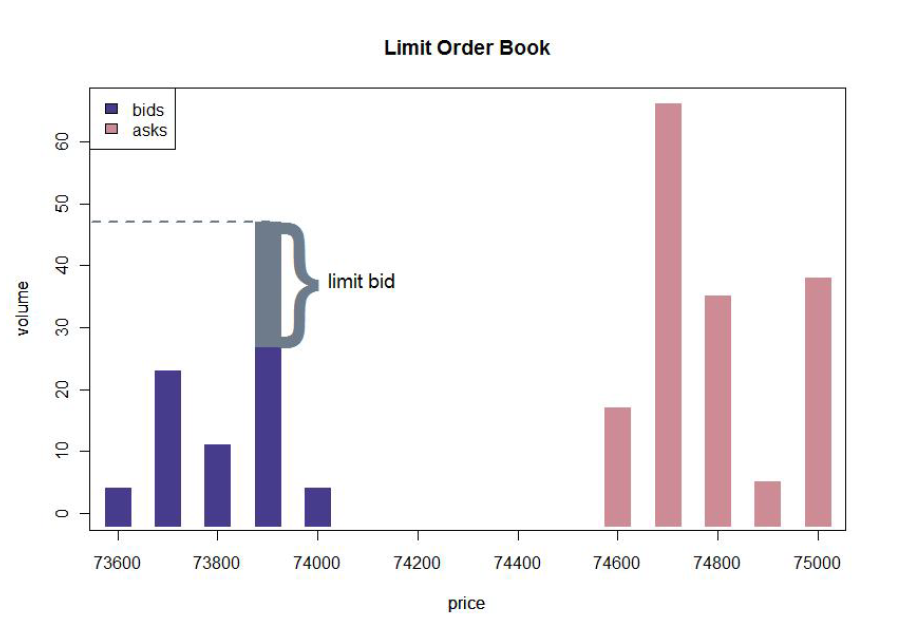
\includegraphics[width=0.9\textwidth]{chapters/chapter_trading_fund/figures/limitbk1.png} 
	   \caption{Limit Order Book---Limit Bid. \label{fig:limbk1}}
	\end{figure}
	
	\begin{figure}[!ht]
	   \centering
	   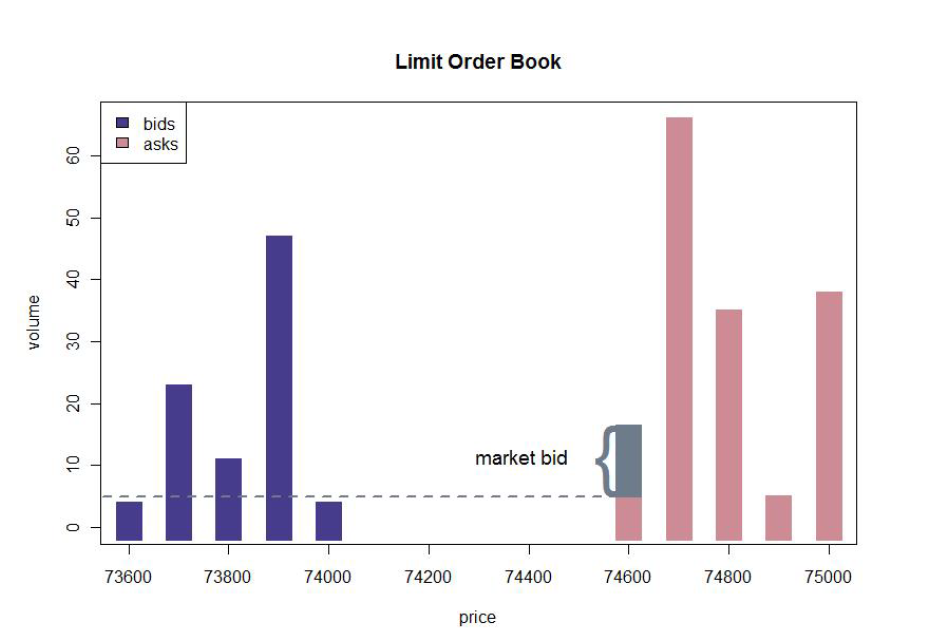
\includegraphics[width=\textwidth]{chapters/chapter_trading_fund/figures/limitbk2.png} 
	   \caption{Limit Order Book---Marketable Bid. \label{fig:limbk2}}
	\end{figure}
	
	
When a market (or marketable) order is submitted, it decreases the number of outstanding orders at the opposite best price. For example, if a market bid order arrives, it will decrease the number of outstanding asks at the best price.
	\begin{figure}[!ht]
	   \centering
	   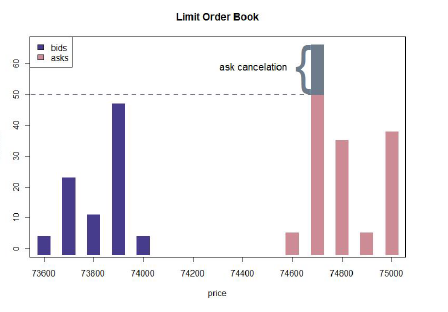
\includegraphics[width=\textwidth]{chapters/chapter_trading_fund/figures/limitbk3.png} 
	   \caption{Limit Order Book---Ask Cancellation. \label{fig:limbk3}}
	\end{figure}
All unexecuted limit orders can be canceled. When a cancellation occurs, it will decrease the number of outstanding orders at the specified price level.


Limit orders make up a significant percentage (70\%) of stock market trading activity. The main advantage of a limit order is that there is no price risk associated to it, that is, when the order is executed the limit price is the maximum (for a buy order) or minimum (for a sell order) price that will be achieved. But if the limit order is not marketable, the execution is not guaranteed and the time to get an order executed depends on various market factors. The trade-off between limit orders and marketable orders depends on the investors need for immediate liquidity and the fill probability of limit orders. The limit price chosen (how deep in the order book is the order placed) as well as the amount of liquidity ahead of the submitted order (how many shares will need to trade before the order gets executed following, for instance, a price/time priority order matching of the exchange) affect both the order fill probability and its expected time to fill. 


These two metrics are of particular relevance for execution algorithms and will be studied in more depth later. The execution of limit orders does affect how the quotes are posted and are updated. If the size of a market order exceeds the number of shares available at the top of book, it is usually split and is executed at consecutive order book levels until the order is filled. Market orders are usually restricted to be filled within a day and order placed after the markets close might be entered the next day.\footnote{Depending on the Time-in-Force selected} \\


\noindent\textbf{Order Types:} The diversity of order types is a key component of continuous double auction electronic markets. Order types allow participants to precisely express their intentions with regards to their interaction with the limit order book. Over time, in an effort to cater to sophisticated electronic traders, exchanges around the world have raced to offer ever more complex order types. Here, we will just provide a brief description of the main ones:

\begin{itemize}
\item  Market: Request to buy or sell immediately at the best available price. While it does not guarantee the trader a price, it guarantees execution. For small order sizes in actively traded stocks, a buy market order would execute close to the best ask price, and a sell order close to the best bid price.

\item  Limit: Specify a maximum (minimum) price at which the trader is willing to buy (sell). If liquidity is available at a better price, the order will execute at that price.

\item  Peg: Specify a price level at which the order should be continuously automatically repriced. For instance, an order pegged to the bid price will be automatically repriced as a higher price limit order each time the market bid price ticks up. This order type is particularly used for midpoint executions in non-displayed markets. One would think that pegging orders has the additional advantage of improving the queue priority of the order when it is repriced since this process is done directly by the exchange. That turns out not to be true. Managing peg orders is responsibility of a separate component at the exchange and it's interaction speed with the order book is usually slower than that of ultra-low-latency operators.

\item  Iceberg: Limit order with a specified display quantity. In order to prevent information leakage to other market participants, a trader desiring to buy or sell a large quantity at a given price might elect to use an iceberg order with a small display size. For instance, for an order to buy 100,000 shares at \$20 with a display size of 2,000 shares, only 2,000 shares would be displayed in the order book. Once that quantity is executed, the order would automatically reload another 2,000 shares at \$20, and so on until the full quantity is executed. Note that for iceberg orders only the visible quantity has time priority and once that quantity has been executed the new tip of the iceberg will be placed at the back of the queue

\item  Hidden: While they are available to trade, these orders are not directly visible to other market participants in the central limit order book. 

\item  Stop: These orders are also not visible, but additionally are not immediately entered in the limit order book. They only become active once a certain price (known as the Stop Price) is reached or passed, then enter the order book as either limit or market order depending on the user setup.

\item  Trailing stop: These orders function like stop orders, but the stop price is dynamic rather than static (for instance: $-3\%$ from previous close).

\item  AON (All-or-None): Specifically, request a full execution of the order. If the order is for 1500 shares but only 1000 are being offered, it won't be executed until the full quantity is available.

\item  OO (On-Open): Specifically, request an execution at the open price. It can be limit-on-open (LOO) or market-on-open (MOO).

\item  OC (On-Close): Specifically, request an execution at the close price. It can be limit-on-close (LOC) or market-on-close (MOC).

\item  IO (Imbalance only): Provide liquidity intended to offset on-open/on-close orders imbalances during the Opening/Closing Cross. These generally must be limit orders.

\item  d-Quote: Special order type on the NYSE mainly used during the close auction period.

\item  Funari: Special order type on the Tokyo Stock Exchange which allows limit orders placed in the book during the continuous session to automatically enter the closing auction as market orders. \\
\end{itemize} 


As described above, there exist a wide variety of orders types offered by different exchanges to facilitate certain types of trading activities. Two additional common order types used to automate interactions with the LOB are stop-limit orders and trailing-stop orders. The former type is typically used to trade a security at a specified limit price once it traded through a given stop price. If the stock declines in value and trades below or at the stop price, the order will become a limit order rather than a market order. Trailing-stop orders follow a similar objective but the stop price trails the best bid or ask by a certain percentage. These order types are primarily used by traders as a protection against sudden adverse market moves. \\


\noindent\textbf{Validity of Instructions:} In addition to conditions on price, it is possible to add conditions on the life duration of the order known as Time-in-Force (TIF). The most common types of TIF instructions include Day orders which are valid for the full duration of the trading session, Extended Day orders which allow trading in extended hours, and Good-Till-Cancel (GTC) orders which will be placed again on the exchange the next day with similar instructions if they were not fully filled. More sophisticated market participants aiming at achieving greater control over their executions tend to also favor Immediate-or-Cancel (IOC) and Fill-or-Kill (FOK) Time-in-Force instructions. An IOC order will get immediately canceled back to the sender after reaching the matching engine if it does not get an immediate fill, and in case of a partial fill, the unfilled portion will be canceled, thus preventing it from creating a new price level in the order book. In a Fill-or-Kill scenario, the order gets either filled in its entirety or does not get filled at all. This instruction is particularly popular with high frequency market makers and arbitrageurs for which partial fills might result in unwanted legging risk as discussed in Chapter~\ref{ch:stat_ts} on pairs trading.


Finally, it is worth mentioning that some exchanges as well as alternative venues offer the ability of specifying minimum fill sizes whereby a limit order which might be eligible for a fill due to an incoming order at the same price level only receives a fill if the incoming order is larger than a pre-specified number of shares or notional value. This type of instruction is used by market participants as a way of minimizing the number of small fills which carry the risk of excessive information dissemination, in particular in dark pools where they can be used to detect the presence of larger limit orders that would otherwise not be visible to market participants.  \\



% The Closing Auction
\subsection{The Closing Auction} 
The Closing Auction tends to be the most popular of call auctions for a variety of interesting reasons. First, it is the last opportunity (unless one engages in the highly risky practice of off-hours trading) for market participants to transact in a relatively liquid environment before being exposed to the overnight period (when new information accumulates, but trades cannot easily take place). Second, with the increase in passive investment strategies providing investors with replication of a predetermined benchmark index, the closing auction has become a particularly relevant price setting event (most passive funds net asset valued (NAV) is based on close prices of the underlying assets). For such reasons, the closing auction is extremely important to many investors. From an execution standpoint, it is a major liquidity event that needs to be considered carefully.


The mechanics of the closing auction are in most part similar to the ones described above for the open auction. The major differences across countries (and sometimes across exchanges within a country) have to do with order submission times. Some countries, such as the U.S., have order submissions start and end before the continuous session is over (see Table~\ref{tab:NASDAQclose} and Table~\ref{tab:NYSEclose}); while some other markets have two non-overlapping continuous and close order submission sessions.

	\begin{table}[!ht]
   	\centering
   	\caption{Nasdaq Closing Cross\label{tab:NASDAQclose}}
   	\begin{tabular}{ll} 
	3:55 p.m. EST & Dissemination of imbalance information begins  \\ \hline
	3:55 p.m. EST & Cutoff for entry/amend/cancel of MOC orders\\ \hline
	3:58 p.m. EST & Freeze period - LOC orders cannot be added/canceled  \\ 
	 & OI orders offsetting the imbalance are still accepted   \\ \hline	
	4:00 p.m. EST & The Closing Cross occurs		
  	 \end{tabular}
	\end{table}	


	\begin{table}[!ht]
   	\centering
   	\caption{NYSE Closing Cross\label{tab:NYSEclose}}
   	\begin{tabular}{ll} 
	3:45 p.m. EST & Cutoff for MOC/LOC order entry and modifications  \\ 
     	& Dissemination of imbalance information begins \\
	& Closing Offset orders can be entered until 4:00 p.m.  \\ \hline	 
	3:55 p.m. EST &  Dissemination of d-quote imbalance information\\ \hline
	3:58 p.m. EST & Cutoff for MOC/LOC cancellation for legitimate error \\ \hline
	3:59:50 p.m. EST & Cutoff for d-Quote order entry and modification \\ \hline
	4:00 p.m. EST & The Closing Auction starts \\ \hline
	4:02 p.m. EST & DMM can automatically process auctions not yet complete
   	\end{tabular}
	\end{table}	


	\begin{table}[!ht]
  	\centering
   	\caption{London Stock Exchange Sessions Times\label{tab:LSEclose}}
   	\begin{tabular}{ll} 
	7:00-7:50 a.m. GMT & Pre-Trading  \\ \hline
	7:50-8:00* a.m. GMT & Opening Auction Call\\ \hline
	*8:00-12:00 p.m. GMT & Regular Trading \\ \hline
	12:00-12:02* p.m. GMT & Periodic Call Auction \\ \hline
	*12:02-4:30 p.m. GMT & Regular Trading \\ \hline
	4:30-4:35* p.m. GMT & Closing Auction Call \\ \hline
	*4:35-4:40 p.m. GMT & Closing Price Crossing \\ \hline	
	4:40-5:15 p.m. GMT & Post-Close Trading
   	\end{tabular}
	\begin{minipage}[t]{1\textwidth}
	\small{*Each auction end time is subject to a random 30 second uncross period.\\}
	\small{An additional intraday auction call takes place every 3rd Friday of each month for stocks underlying FTSE 100 index options, and the 3rd Friday of every quarter for stocks underlying FTSE 100/250 Index Futures to determine the EDSP (Exchange Delivery Settlement Price). The settlement price is determined as the index value derived from the individual constituents intraday auction taking place between 10 a.m. and 10:15 a.m. and during which the electronic continuous trading is suspended. Using a call auction ensures the settlement price for these contracts is more representative of a fair market price.}
	\end{minipage}   
	\end{table}	


One specificity of the NYSE is the presence of floor brokers operating in an agency capacity for their customers. They play a particular role during the close auction thanks to their ability to handle discretionary electronic quote orders (known as ``d-Quote'' orders) that offer more flexibility than traditional MOC and LOC orders. The main advantage of d-Quote orders is their ability to bypass the 3:45 pm cutoff and be submitted or canceled until 3:59:50 pm. This allows large institutional investors to remain in control of their orders almost until the end of the continuous session by delaying the decision of how much to allocate to the auction. They can therefore react to larger volume opportunities based on the published imbalance, but also minimize their own information leakage by not being part of the early published imbalance while there is still significant time in the continuous session for other participants to drive the price away.  Since there is no restriction on the side of d-Quote orders submission, it is possible to see the total imbalance sign flip once the d-Quotes are added to the publication at 3:55 pm, creating opportunities for other market participants to adjust their own close trading via d-Quotes or change their positioning in the continuous session. \\



% Taxonomy of Data for Algorithmic Trading Research
\section{Taxonomy of Data used in Algorithmic Trading }

To run a successful trading operation in particular for it's more research oriented aspects requires availability of lot of different data sets. Data availability, storage, management, cleaning are some of the most important aspect of a functioning trading business and the core of any research environment. The amount of data and the complexity of maintaining the ``Data Lake'' can be daunting and very few  excel at this aspect.

In this section we'll review the most important data sets and their role in AT research.

\begin{comment}
Historical market data available to researchers and practitioners alike but varied in degrees of granularity over time. From daily trade data (closing price and volume), to tick-by-tick trade and quote data (also known as TAQ data), to full message data, the progression in granularity not only reflects the focus in intraday trading complexity but also opens up the way for more advanced strategies. 


Initially researchers studying the dynamic of LOB had to be content with Trades and Quotes (TAQ) data which provide a time-stamped sequence of trades (Market Orders) and updates in the price and depth of bid and ask quotes. No other information beyond the best bid and the best offer was made available. Also, the updates contained changes at the two best quotes and were aggregated. The aggregation was clearly a limiting factor as one could not discern the kind of events that led to the changing status of the book. The level II data that became available is a time-stamped sequence of trades and quotes for the top 5-levels of the LOB. This data is little deeper than TAQ data, but was still in aggregated form. But recently made available level III data contains time-stamped sequence of all (except for the submission of hidden orders) events that occur in the LOB. Every order is identified by a unique order-id and thus it can be tracked through its lifetime.\footnote{Level III data has been available for years to firm subscribing and storing the raw binary exchange format (pcap) and the re-building the orderbook sequentially from there for their research. It is still the main method used for HFT research. One recently this data became available historically to a broader subset of users and researchers} \\
\end{comment}


% Reference Data
\subsection{Reference Data} 

While often overlooked, or merely considered as an afterthought in the development of a research platform,\footnote{More details are presented in a further chapter on research environment} reliable reference data is the key foundation of a robust quantitative strategy development. The experienced practitioner might want to skip this section, however we encourage the neophyte to read through the tedious details to get a better grasp of the complexity at hand in the
different categories of reference data.


\begin{itemize}
\item \textbf{Trading Universe:}

The first problem for both the correct functioning of a trading operation is knowing what instruments you will be required to trade on a particular day. The trading universe is an ever evolving entity that changes daily to incorporate new IPOs, listings, de-listings, etc. To be able to just trade a new instruments there are several pieces of information that one is required to have in multiple systems. Market Data needs to be available, and some staict data needs to be set or guessed to work with existing controls, parameters for the various analytics need to be available or sensibly defaulted.

For research, in particular quantitative strategies, knowing when a particular stock no longer trades is important to avoid issues like survivor bias.
 
\item \textbf{Symbology Mapping:} ISIN, SEDOL, RIC, Bloomberg Tickers, \dots

Quantitative strategies often leverage data from a variety of sources. Different providers key their data with different instrument identifiers depending on asset class or regional conventions, or sometime use their own proprietary identifiers (e.g. Reuters Identification Code---RIC, Bloomberg Ticker), therefore making symbology mapping the first step in any data merging exercise. Such data is not static, one of the symbols can change on a given day and others remain unchanged for some time, complicating historical data merges.


It is important to note that such mapping needs to be persisted as point-in-time data and allow for historical ``as of date'' usage. Over the course of time, some instruments undergo ticker changes (for example from ABC to EDF on a later $T_0$.) without necessarily any particular change on the underlying asset. In such cases, market data recorded day-by-day in a trade database will change from being keyed on ABC to being keyed on EDF after the ticker change date $T_0$. This has large implications for practitioners working on datasets to build and backtest quantitative strategies. The symbology mapping should allow both backward and forward handling of the changes.


For instance, in the simple example mentioned, in order to efficiently backtest strategies over a period of time spanning $T_0$, one needs a robust mapping that will allow to seamlessly query the data for the underlying asset in a variety of scenarios such as:

\begin{itemize}
\item Signal generation: 30-day backward close time series as of date $T < T_0$: \par
{\ttfamily select close from data where date in [T-30,  T], sym = ABC}

\item Signal generation: 30-day backward close time series as of date $T= T_0+10$: \par
{\ttfamily select close from data where date in [T$_0$ - 20, T$_0$ + 10], sym = EDF}

\item Position holding: 30-day forward close time series as of date $T= T_0-10$: \par
{\ttfamily select close from data where date in [T$_0$ - 10,  T$_0$ + 20], sym = ABC}
\end{itemize}


\item \textbf{Ticker Changes:} For comparable reasons as the ones described above in the Symbology Mapping section, one needs to maintain a historical table of ticker changes allowing to seamlessly go up and down time series. 


\item \textbf{Corporate Actions Calendars:} This category contains stock and cash dividends (both announcement date and execution date), stock splits, reverse splits, rights offer, mergers and acquisitions, spin off, free float or shares outstanding adjustments, quotation suspension.


Corporate actions impact the continuity of price and volume time series and, as such, need to be recorded in order to produce adjusted time series. The most common events are dividend distributions. On the day the dividend is paid, the corresponding amount is removed from the stock price, creating a jump in the price time series. The announcement date might also see the stock experience added volatility as investors react to the news. Consequently, recording these events proves to be valuable in the design of quantitative strategies as one can assess the effect on performance of dividends announcement or payment, and decide to either not hold a security that has an upcoming dividend announcement or, conversely, to build strategies that look to benefit from the added volatility. 


Additional types of corporate actions generating discontinuity in historical time series are stock splits or reverse splits and right offers. When the price of a stock becomes either too low or too high, a company might seek to split it to bring the price back to a level that is more conducive to liquid trading on exchanges\footnote{A very low price creates trading frictions as the minimum price increment might represent a large cost relative to the stock price. A very high price might also deter retail investors from investing into a security as it requires them to deploy too much capital per unit.}. When a stock experiences a 2:1 split, everything else being equal, its price will be halved and its volume will double. In order to prevent the time series to show a 50\% drop in price, all historical data will then need to be adjusted backward to reflect the split.


Mergers \& Acquisitions and Spin-offs are also regular events in the lifecycle of corporations. Their history needs to be recorded in order to account for the resulting changes in valuation that might affect a given ticker or tickers. These situations can also be exploited by trading strategies known as Merger Arbitrage.


Stocks quotation can be suspended as a cooling mechanism (often at the request of the underlying company) to prevent excess price volatility when significant information is about to be released to the market. Depending on the situation, the suspension can be temporary and intraday, or can last for extended periods of time if the market place allows it.\footnote{For instance, it was the case for a large number of companies in China in 2016.} Suspensions result in gaps in time series and are worth keeping track of, as they can impact strategies in backtesting (inability to enter or exit a position, uncertainty in the pricing of composite assets if a given stock has a significant weight in ETFs or Indexes). Some markets will also suspend trading if the price swings more than a predefined amount (limit up / limit down situations) for either a period of time or for the remainder of the trading session.


\item \textbf{Static Data:} Country, sector, primary exchange, currency and quote factor.


Pure static data is also relevant for the development of quantitative trading strategies. In particular, country, currency and sector are useful to group instruments based on their fundamental similarities. A well known example is the usage of sectors to group stocks in order to create pairs trading strategies. It is worth mentioning that there exist different types of sector classifications (e.g. GICS\textsuperscript\textregistered from S\&P, ICB\textsuperscript\textregistered from FTSE) offering several levels of granularity,\footnote{The Global Industry Classification Standard (GICS\textsuperscript\textregistered) structure consists of 11 sectors, 24 industry groups, 68 industries and 157 sub-industries. An example of this hierarchical structure would be: Industrials / Capital Goods / Machinery / Agricultural \& Farm Machinery.} and that different classifications might be better suited to different asset classes or countries. The constituents of the Japanese index TOPIX, for instance, are classified into 33 sectors that are thought to better reflect the fundamental structure of the Japanese economy and the existence of large diversified conglomerates. 


Maintaining a table of the quotation currency per instrument is also necessary in order to be able to aggregate positions at a portfolio level. Some exchanges allow the quotation of prices in currencies different from the one of the country in which the exchange is located.\footnote{For example, Jardine Matheson Holdings quotes in USD on the Singapore exchange while most of the other securities quote in Singapore Dollars.} Additionally, the Quote Factor associated with the quotation currency data needs to be stored. To account for the wide range of currency values and preserve pricing precision, market data providers might be publishing FX rates with a factor of 100 or 1000. Hence, to convert prices to USD one needs to multiply by the quote factor: usd price $=$ local price $\cdot$ fx $\cdot$ quote factor. Similarly, some exchanges quote prices in cents, and the associated quotation currency is reflected with a small cap letter: GBP/GBp, ZAR/ZAr, ILS/ILs, \dots).


\item \textbf{Exchange Specific Data:}  Despite the electronification of markets, individual exchanges present a variety of differences that need to be accounted for when designing trading strategies. The first group of information concerns the hours and dates of operation:

\begin{itemize}
\item Holiday calendar: As not all exchanges are closed on the same day, and trading days off do not always fully follow the country public holidays, it is valuable to record them in particular in the international context. Strategies trading simultaneously in several markets and leveraging their correlation might not perform as expected if one of the markets is closed while the others are open. Similarly, execution strategies in one market might be impacted by the absence of trading in another market (for instance, European equity markets volume tends to be 30\% to 40\% lower during U.S. market holidays).

\item Exchange sessions hours: These seemingly trivial data points can get quite complex on a global scale. What are the different available sessions (Pre-Market session, Continuous core session, After-Hour session, etc.)? What are the auction times as well as their respective cutoff times for order submission? Is there a lunch break restricting intraday trading? And if so, are there auctions before and after the lunch break? \dots Futures markets sessions can also be quite complex with multiple phases, breaks, as well as official settlement times that might differ from the closing time and have an effect on liquidity.

In Indonesia, for instance, markets have different trading hours on Fridays. Monday through Thursday the Indonesia Stock Exchange (IDX) is open from 9:00~a.m. to 12:00~p.m., and then, from 1:30~p.m. to 4:00~p.m.. On Fridays, however, the lunch break is one hour longer and stretches from 11:30~a.m. to 2:00~p.m.. This week day effect is particularly important to consider when building volume profiles as described in Chapter~\ref{ch:stat_ts}.

Along with local times of operation, it is necessary to consider eventual Daylight Saving Time (DST) adjustments that might effect the relative trading hours of different markets (some countries do not have DST adjustment at all, while for countries that do have one, the dates at which it applies are not always coordinated). Usually, DST starts about two weeks prior to its start in Europe, bringing the time difference between New York and London to 4~hours instead of 5~hours. This results in the volume spike in European equities associated to the U.S. market open being one hour earlier, requiring adjustment of volume profiles used for trading execution.

Some exchanges might also adjust the length of trading hours during the course of the year. In Brazil for instance, the Bovespa trading hours are 10:00~a.m. to 6:00~pm. from October to March, but an hour shorter (10:00~a.m. to 5:00~p.m.) from April to September to be more consistent with U.S. market hours. Finally, within one country there might also exist different trading hours by venues as it is the case in Japan where the Nagoya Stock Exchange closes 30~minutes after the major Tokyo Stock Exchange.

\item Disrupted days: Exchange outages or trading disruptions, as well as market data issues, need to be recorded so they can be filtered out when building or testing strategies as the difference in liquidity patterns or the lack of data quality might impact the overall outcome.
\end{itemize}


Additionally, exchanges also have specific rules governing the mechanics of trading, such as:
        \begin{itemize}
        \item Tick Size: The minimum eligible price increment. This can vary by instrument, but also change dynamically as a function of the price of the instrument (e.g. stocks under \$1 can quote in increments of \$0.0001, while above that price the minimum quote increment is \$0.01).
        \item Trade and Quote lots: Similarly to tick sizes, certain exchanges restrict the minimum size increment for quotes or trades.
        \item Limit-up and Limit-down constraints: A number of exchanges restrict the maximum daily fluctuations of securities. Usually, when securities reach these thresholds, they either pause trading or can only be traded at a better price than the limit-up limit-down threshold.
        \item Short Sell restrictions: Some markets also impose execution level constraints on short sells (on top of potential locate requirements). For instance, while a long sell order can trade at any price, some exchanges restrict short sells to not trade at a price worse than the last price or not create a new quote that would be lower than the lowest prevailing quote. These considerations are particularly important to keep in mind for researchers developing Long-Short strategies as this impacts the ability to source liquidity.
        \end{itemize}
Because these values and their potential activation threshold can vary over time, one needs to maintain historic values as well in order to run realistic historical backtests.


\item \textbf{Market Data Condition Codes:} With ever-growing complexity in market microstructure complexity, the dissemination of market data has grown complex as well. While it is possible to store daily data as a single entry per day and per instrument, investors building intraday strategies likely need to collect tick by tick data of all the events occurring in the market place. To help classify events, exchanges and market data providers attribute so-called condition codes to the trades and quotes they publish. These condition codes vary per exchange and per asset class, and each market event can be attributed several codes at once. So, to aggregate intraday market data properly and efficiently, and decide which events to keep and which ones to exclude, it is necessary to build a mapping table of these condition codes and their meaning: auction trade, lit or dark trade, cancelled or corrected trade, regular trade, off-exchange trade reporting, block-size trade, trade originating from a multi-leg order such as an option spread trade, \dots


For instance, in order to assess accessible liquidity for a trading algorithm, trades that are published for reporting purposes (e.g. negotiated transactions that happened off-exchange) need to be excluded. These trades should also not been used to update some of the aggregated daily data used in the construction of trading strategies (daily volume, high, low, \dots). Execution algorithms also leverage extensively distribution of intraday liquidity metrics to gauge their own participation in auctions and continuous sessions, or in lit versus dark venues, therefore requiring a precise classification of intraday market data. 


\item \textbf{Special Day Calendars:} Over the course of a year, certain days present liquidity characteristics that need to be accounted for in both execution strategies and in the alpha generation process. The diversity of events across markets and asset classes can be quite challenging to handle here as well. Among the irregular events that affect liquidity in equity markets and need to be accounted for, we can mention the following non-exhaustive list for illustration purposes: half trading days preceding Christmas and following Thanksgiving in the U.S. or on the Ramadan eve in Turkey, Taiwanese market opening on the weekend to make up for lost trading days during holiday periods, Korean market changing its trading hours on the day of the nationwide university entrance exam, Brazilian market opening late on the day following the Carnival, etc..


There are also special days that are more regular and easier to handle. The last trading days of the months and quarters, for instance, tend to see additional trading activity as investors rebalance their portfolios. Similarly, options and futures expiry days (quarterly/monthly expiry, `Triple Witching'\footnote{Triple witching days happen four times a year on the third Friday of March, June, September and December. On these days, the contracts for stock index futures, stock index options and stock options expire concurrently.} in the U.S., Special Quotations in Japan, etc.) tend to also have relative excess trading volume and different intraday patterns resulting from hedging activity and portfolios adjustments. Consequently, they need to be handled separately, in particular when modeling trading volume. As most execution strategies make use of relatively short interval volume metrics (e.g. 30-day or 60-day ADV), one single data point can be enough to impact the overall level inferred. Similarly autoregressive models of low order might underperform both on special days and on the days following them. As a result, modelers often opt for removing special days from data sets and model normal days first. Then, special days are modeled separately, either independently or using the normal days as a baseline. 


In order to reflect changes in the market and remain consistent with index inclusion rules, most indexes need to undergo regular updates of their constituents as well as their respective weights. The significant indexes do so at regular intervals (annually, semi-annually or quarterly) on a pre-announced date. At the close of business of that day, some stocks might be added to the index while others are removed, or the weight of each stock in the index might be increased or decreased. These events, known as index rebalances, are particularly relevant to passive investors who are tracking the impacted index. In order to minimize the tracking error to their benchmark index, they need to also adjust their holdings accordingly. Additionally, as most funds are benchmarked at the close price, there is an incentive for fund managers to try to rebalance their holdings at a price as close as possible to the official close price on the day the index rebalance becomes effective. As a result, on these days, intraday volume distribution is significantly skewed toward the end of day and requires adjustment of execution strategies.


It is worth noting that a special day calendar usage needs not be limited to the country where the event occurs. On days when the U.S. Equities market is closed, there is usually also a significant drop in volume traded in European markets, so it is always valuable to investigate the cross market effect of special days.


\item \textbf{Futures-specific Reference Data:} Futures contracts present particular characteristics requiring additional reference data to be collected. One of the core differences of futures contracts compared to regular stocks is the fact that instruments have an expiry date, after which they cease to exist. For the purpose of backtesting strategies, it is necessary to know which contract was live at any point in time through the use of an expiry calendar, but also which contract was the most liquid (for instance, equity index futures tend to be the most liquid for the first contract available (also known as front month) while energy futures such as oil tend to be more liquid for the second contract. While this may appear to be trivial, when building a trading strategy and modeling price series, it is particularly important to know which contract carries the most significant price formation characteristics and what is the true liquidity available in order to estimate transaction costs to properly estimate the market impact. 


The task of implementing a futures expiry calendar is further complicated by the fact there is no real standardized frequency that applies across markets. For instance, European equity index futures tend to expire monthly, while U.S. index futures expire quarterly. Some contracts even follow an irregular cycle through the course of the year as it is the case for grain futures (e.g. wheat) that were originally created for hedging purposes and as a result have expiry months that follow the crop cycle.\footnote{U.S. Wheat Futures expire in March, May, July, September and December}


The fact futures contracts expire on a regular basis has further implications in terms of liquidity. As investors holding these contracts, they want to maintain their exposure for longer than the lifespan of the contract, they need to roll over their positions onto the next contract. There is often a noticeable difference in the liquidity of consecutive contracts (for instance, the front contract of the S\&P500 (e.g. ESH8) trades roughly 1.5 million contracts per day in the weeks preceding expiry while the next month contract (ESM8) only trades about 30,000 contracts per day). However, this liquidity relationship will invert in the few days leading to the expiry of the front contract as most investors roll their positions, and the most liquid contract will become the back month contract (see Figure~\ref{fig:FutRoll}). As a result, when computing rolling-window metrics (such as average daily volume for instance), it is necessary to account for potential roll dates that might have happen during the span of the time series. In the example above, a simple 60-day average daily volume on ESM8 taken in early April 2018 would capture a large number of days with very low volume (January-March) owing to the fact the most liquid contract at the time was the ESH8 contract, and not accurately represent the volume activity of the S\&P500 futures contract. A more appropriate average volume metric to be used as a forward looking value for execution purposes would blend the volume time series of ESH8 prior to the roll date, and ESM8 after the roll date.\footnote{It is worth noting that different contracts 'roll' at different speed. While for monthly expiry contracts it is possible to see most of the open interest switch from the front month contract to the back month on the day prior to the expiry, for quarterly contracts it is not uncommon to see the roll happen over the course of a week or more, and the front month liquidity vanish several days ahead of the actual expiry. Careful modeling is recommended on a case by case basis.} Additionally, in order to efficiently merge futures positions with other assets in an investment strategy, one needs to store reference data relative to the quotation of these contracts: contract size (translation between the quotation points and the actual monetary value), currency, etc. 

	\begin{figure}[!ht]
	\centering
	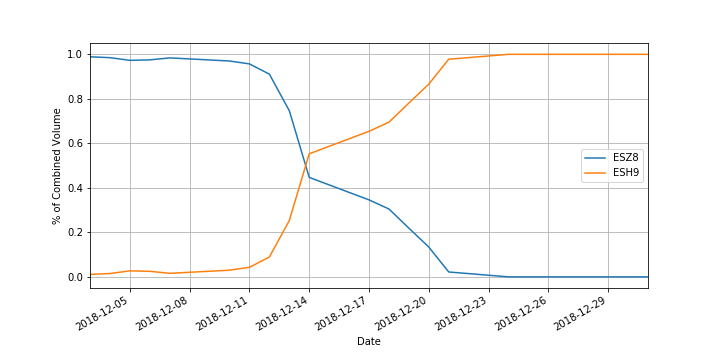
\includegraphics[width=\textwidth]{chapters/chapter_trading_fund/figures/FutRoll.png} 
	\caption{Futures Volume Rolling. \label{fig:FutRoll}}
	\end{figure}

Finally, futures markets are characterized by the existence of different market phases during the day, with significantly different liquidity characteristics. For instance, equity index futures are much more liquid during the hours when the corresponding equities markets are open. However, one can trade during the overnight session if they need to. The overnight session being much less liquid, the expected execution cost tends to be higher, and as such, the various market data metrics (volume profile, average spread, average bid-ask sizes, ...) should be computed separately for each market phase, which requires maintaining a table of the start and end times of each session for each contracts. 


\item \textbf{Options-specific Reference Data (Options Chain):} Similar to futures contracts, options contracts present a certain number of specificities for which reference data need to be collected. On top of the similar feature of having a particular expiry date, options contracts are also defined by their strike price. The combination of expiries and strikes is known as the the option chain for a given underlier. The ability to map equity tickers to options tickers and their respective strike and expiry dates allows for the design of more complex investment and hedging strategies. For instance, distance to strike, change in open interest of puts and calls, etc. can all be used as signals for the underlying security price.


\item \textbf{Market-Moving News Releases:} Macro-economic announcements are known for their ability to move markets substantially. Consequently, it is necessary to maintain a calendar of dates and times of their occurrences in order to assess their impact on strategies and decide how to best react to them. The most common ones are central banks announcements or meeting minutes releases of the major economies (FED/FOMC, ECB, BOE, BOJ, SNB), Non-Farm Payrolls, PMI, Crude Oil Inventories, etc.. While these news releases impact the broad market or some wide sectors, there are also stock specific releases that need to be tracked: earning calendars, specialized sector events such as FDA results for the healthcare and biotech sectors\dots 


\item \textbf{Related tickers:} There is a wide range of tickers that are related to each other, often because they fundamentally represent the same underlying asset. Maintaining proper reference allows to efficiently exploit opportunities in the market. Some non-exhaustive examples include: primary tickers to composite tickers mapping (for markets with fragmented liquidity), dual listed/fungible securities in US and Canada, American Depository Receipt (ADR) or Global Depository Receipt (GDR), local and foreign boards in Thailand, \dots 


\item \textbf{Composite Assets:} Some instruments represent several underlying assets (ETFs, Indexes, Mutual Funds, \dots). Their rise in popularity as investments over time makes them relevant for quantitative strategies as they can be used as efficient vehicles to achieve desired exposures (sector and country ETFs, thematic factor ETFs, \dots), can be used as cheap hedging instruments, can provide arbitrage opportunities when they deviate from their Net Asset Value (NAV), and so on. 
In order to be leveraged in quantitative strategies, one needs to maintain a variety of information such as a time series of their constituents and the value of any cash component, a time series of the divisor used to translate the NAV into the quoted price, a time series of constituent weights. 


\item \textbf{Latency tables:} This last type of data would only be of interest for strategies and research in the higher frequency trading space. For these, it might be relevant to know the distribution of latency between different data centers as they can be used for more efficient order routing as well as reordering time series that may have been recorded in different locations.
\end{itemize}


While the points mentioned above represent a non-exhaustive list of the reference data available to build a quantitative research platform, they highlight the challenges that need to be taken into account when designing and implementing algorithmic trading strategies. Once in place, a proper set of reference data will allow the quantitative trader to systematically harness the actual content of the types of data described later on without being caught off-guard by the minutiae of trading.\\







% Raw Market Data
\subsection{Market Data} 
While historically a large swath of modeling was carried out on daily data or minute bar datasets, the past fifteen years have seen a significant rise in the usage raw market data in an attempt to extract as much information as possible, and act on it before the opportunity (or market inefficiency) dissipates.


Market data, itself, comes in various levels of granularity (and price!) and can be subscribed to either directly from exchanges (known as ``direct feeds'') or from data vendors aggregating and distributing it. The level of detail of the feed subscribed to is generally described as Level I, Level II or Level III market data.\\


\noindent\textbf{Level I data: Trade and BBO Quotes:} Level I market data is the most basic form of tick-by-tick data. Historically, the level I data feed would only refer to trade information (Price, Size, Time of each trade reported to the tape) but has grown over time into a term generally accepted to mean both trades and top of book quotes. While the trade feed updates with each trade printed on the tape, the quote feed tends to update much more frequently each time liquidity is added to or removed from the top of book (a rough estimate in liquid markets is the quotes present more updates than the trades by about an order of magnitude). 


In order to build strategies, the timing of each event needs to be as precise as possible. While the time reported for trade and quotes is the matching engine time at the exchange, most databases also store a reception or record time to reflect the potential latency between the trade happening and one being aware it did happen and able to start making decision on it. Accounting for this real-world latency is a necessary step for researchers building strategies on raw market data for which opportunities might be very short lived and impossible to exploit by participants who are not fast enough.


The Level I data is enough to reconstruct the Best Bid and Offer (BBO) of the market. However, in fragmented markets, it is also useful to obtain an aggregated consolidated view of all available liquidity at a given price level across all exchanges. Market data aggregator usually provide this functionality for users who do not wish to reconstruct the full order book themselves. 


Finally, it is worth noting that even Level I data contains significant additional information in the form of trade status (cancelled, reported late, etc.) and, trade and quote qualifiers. These qualifiers provide granular details such as whether a trade was an odd lot, a normal trade, an auction trade, an Intermarket Sweep, an average price reporting, on which exchange it took place, etc. These details can be used to better analyze the sequence of events and decide if a given print should be used to update the last price and total volume traded at that point in time or not. For instance, if not processed appropriately, a trade reported to the tape out of sequence could result in a large jump in price if the market has since moved, and consequently the trade status is an indication that the print should not be utilized as is.


Capturing raw market data, whether to build a research database or process it in real-time to make trading decisions requires significant investments and expert knowledge to handle all the inherent complexity. Hence, one should carefully consider the trade off between the expected value that can be extracted from the extra granularity, and the additional overhead compared to simpler solutions such as bin data. \\


\noindent\textbf{Level II data: Market Depth:}  Level~II market data contains the same information as Level I, but with the addition of quote depth data. The quote feed displays all lit limit order book updates (price changes, addition or removal of shares quoted) at any level in the book, and for all of the lit venues in fragmented markets. Given the volume of data generated and the decreasing actionable value of quotes updates as their distance to top of book increases, some users limit themselves to the top 5 or 10 levels of the order book  when they collect or process the data. \\


\noindent\textbf{Level III data: Full Order View:} Level~III market data---also known as message data---provides the most granular view of the activity in the limit order book. Each order arriving is attributed a unique ID which allows for its tracking over time, and precisely know when it is executed, canceled or amended. Similar to Level II, the dataset contains intraday depth of book activity for all securities on an exchange. Once all messages from different exchanges are consolidated into one single dataset ordered by timestamp, it is possible to build a full national depth book at any moment intraday. For illustration purposes, we take the example of U.S. Level III data and provide a short description below and in Table~\ref{tab:level3data}.
	\begin{table}[!ht]
	\centering
	\caption{Level III data \label{tab:level3data}}
	\begin{tabular}{lp{0.8\textwidth}} \hline
	Variable & Description \\
	& \\
	Timestamp: & Number of milliseconds after the midnight. \\
	& \\
	Ticker: & Equity symbol (up to 8 characters) \\
	& \\
	Order: & Unique order ID. \\
	& \\
	T & Message type. Allowed values: \newline \begin{minipage}[t]{0.6\textwidth} \begin{itemize} \item ``B''---Add buy order \item ``S''---Add sell order \item ``E''---Execute outstanding order in part \item ``C''---Cancel outstanding order in part \item ``F''---Execute outstanding order in full \item ``D''---Delete outstanding order in full \item ``X''---Bulk volume for the cross event \item ``T''---Execute non-displayed order \end{itemize} \end{minipage} \\
	& \\
	Shares & Order quantity for the ``B'', ``S'', ``E'', ``X'', ``C'', ``T'' messages. Zero for ``F'' and ``D'' messages. \\
	& \\
	Price & Order price, available for the ``B'', ``S'', ``X'' and ``T'' messages. \newline Zero for cancellations and executions. The last 4 digits are decimal digits. The decimal portion is padded on the right with zeros. The decimal point is implied by position; it does not appear inside the price field. Divide by 10000 to convert into currency value. \\ 
	& \\
	MPID & Market Participant ID associated with the transaction (4 characters) \\
	& \\
	MCID & Market Center Code (originating exchange---1 character) 
	\end{tabular}
	\end{table}
	

While the display and issuance of new ID to the modified order varies from exchange to exchange, a few special types of orders are worth mentioning:
        \begin{enumerate}[1.]
        \item Order subject to price sliding: The execution price could be one cent worse than the display price at NASDAQ; it is ranked at the locking price as a hidden order, and displayed at the price one minimum price variation (normally 1 cent) inferior to the locking price. New order ID will be used if the order is replaced as a display order. At other exchanges the old order ID will be used.
        \item Pegged order: Based on NBBO, not routable, new time stamp upon re-pricing, display rules vary over exchanges.
        \item Mid-point peg order: Non-displayed, can result in half-penny execution.
        \item Reserve order: Displayed size is ranked as a displayed limit order and the reserve size is behind non-displayed orders and pegged orders in priority. The minimum display quantity is 100 and this amount is replenished from the reserve size when it falls below 100 shares. A new timestamp is created and the displayed size will be re-ranked upon replenishing.
        \item Discretionary order: Displayed at one price while passively trading at a more aggressive discretionary price. The order becomes active when shares are available within the discretionary price range. Ranked last in priority. The execution price could be worse than the display price.
        \item Intermarket sweep order: Order that can be executed without the need of checking the prevailing NBBO.  
        \end{enumerate}


The richness of the dataset allows sophisticated players such as market makers to know not only the depth of book at a given price and the depth profile of the book on both sides, but more importantly the relative position of an order from the top position of the side (buy or sell).Among the most common granular microstructure behaviors studied with Level III data, we can mention:
        \begin{itemize}
        \item The pattern of inter-arrival times of various events.
        \item Arrival and cancellation rates as a function of distance from nearest touch price.
        \item Arrival and cancellation rates as a function of other available information, such as in the queue on either side of the book.
        \end{itemize}
Once modeled, these behaviors can, in turn, be employed to design more sophisticated strategies by focusing on trading related questions:
        \begin{itemize}
        \item What is the impact of market order on the limit order book?
        \item What are the chances for a limit order to move up the queue from a given entry position?
        \item What is the probability of making the spread?
        \item What is the direction of the price movement in short duration?\\
        \end{itemize}


As illustrated by the diversity and granularity of information available to traders, markets mechanics have grown ever more complex over time, and a great deal of peculiarities (in particular at the reference data level) need to be accounted for in order to design robust and well performing strategies. The proverbial devil is in the details when in comes to quantitative trading but while it might be tempting to go straight to the most granular source of data, in practice---with the exception of truly high frequency strategies---most practitioners build their algorithmic trading strategies relying essentially on binned data. This simplifies the data collection and handling processes and also greatly reduces the dimension of the datasets so one can focus more on modeling rather than data wrangling. Most of the models and techniques described in subsequent chapters are suited to daily or binned data.

% Market Data Derived Statistics
\subsection{Market Data Derived Statistics}

Most Quantitative strategies even the higher frequency that leverage more and more granular data,leverage derived statistics both at the daily level and binned data. Here we give a list of the most common ones used by practitioners and researchers alike.\\


\noindent\textbf{Daily Statistics}\\
The first group represents the overall trading activity in the instrument: 

\begin{itemize}
\item \emph{High, Low, Close (OHLC) and Previous Close Price:} The OHLC provides a good indication of the trading activity as well as the intraday volatility experienced by the instrument. The distance traveled between the lowest and highest point of the day usually gives a better indication of market sentiment than the simple close-to-close return. Keeping the previous close value as part of the same time series is also a good way to improve computation efficiency by not having make an additional database query to compute intraday return and overnight gap. The previous close needs, however, to be properly adjusted for corporate actions and dividends. 


\item \emph{Last trade before close (Price/Size/Time):} It is useful in determining how much the close price might have jumped in the final moments of trading, and consequently, how stable a reference value it might be for the next day.


\item \emph{Volume:} It is another valuable source of trading activity indication, in particular when the level jumps from longer term average. It is also worth collecting the breakdown between lit and dark volume, in particular for execution strategies.


\item \emph{Auctions volume:} Depending on the exchange, there can be multiple auctions in a day (Open, Close, Morning Close and Afternoon Open - for markets with a lunch break -, as well as adhoc liquidity or intraday auctions). Owing to their liquidity aggregation nature, they often time can be considered as a valuable price discovery event when significant volume prints.


\item \emph{VWAP:} Similar to the OHLC, the intraday VWAP price gives a good indication of the trading activity on the day. It is not uncommon to build trading strategies using VWAP time series instead of just close-to-close prices. The main advantage being that VWAP prices represent a value over the course of the whole day and, as such, for larger orders are easier to achieve through algorithmic execution than a single print.


\item \emph{Short Interest / days-to-cover / utilization:} This dataset is a good proxy for investors positioning. The short pressure might be an indication of upcoming short term moves: a large short interest usually indicates a bearish view from institutional investors. Similarly, the utilization level of available securities to borrow (in order to short) gives an indication of how much room is left for further shorting (when securities become ``Hard to Borrow'', the cost of shorting becomes significantly higher requiring short seller to have strong enough beliefs in the price direction in the short term. Finally, days-to-cover data is also valuable to assess the magnitude of a potential short squeeze. If short sellers need to unwind their positions, how much volume does this represent as a fraction of available daily liquidity. The larger the value, the larger the potential sudden upswing on heavily shorted securities.


\item \emph{Futures data:} Futures markets provide additional insight into the activity of large investors through open interest data that can be useful to develop alpha strategies. Additionally, financial futures offer arbitrage opportunities if their basis exhibits mispricing compared to one's dividend estimates. As such, recording the basis of futures contracts is worthwhile even for strategies that don't particularly target futures.


\item \emph{Index-level data:} This is also a valuable dataset to collect as a source of relative measures for instrument specific features (Index OHLC, Volatility, \dots). In particular for dispersion strategies, normalized features help identify individual instruments from their benchmark. 


\item \emph{Options data:} The derivatives market is a good source of information about the positioning of traders (through open interest and Greeks such as Gamma and Vega) as well as how the broader market is pricing an instrument (through implied volatility for instance).


\item \emph{Asset Class Specific:} There is a wealth of cross-asset information available when building strategies, in particular in Fixed Income, FX, and Credit. Among the basic ones, we would note:
        \begin{itemize}
        \item Yield / benchmark rates (repo, 2y, 10y, 30y)
        \item CDS Spreads
        \item US Dollar Index
        \end{itemize}
\end{itemize}


The second group of daily data represents granular intraday microstructure activity and is mostly of interest to intraday or execution trading strategies:
        \begin{itemize}
        \item \emph{Number of trades:} A proxy for the activity level of an instrument, and how continuous it is (instruments with a low number of trades are harder to execute and can be more volatile). 
        
        \item \emph{Number and frequency of quote updates:} Similar proxy for the activity level.
        
        \item \emph{Top of book size:} A proxy for liquidity of the instrument (larger top of book size make it possible to trade larger order size quasi immediately if needed).
        
        \item \emph{Depth of book (price and size):} Similar proxy for liquidity.
        
        \item \emph{Spread size (average, median, time weighted average):} This provides a proxy for cost of trading. A parametrized distribution of spread size can be used to identify cheap or expensive intraday trading opportunities.
        
        \item \emph{Trade size (average, median):} Similar to spread size, trade sizes and their distribution are useful to identify intraday liquidity opportunities when looking at the volume available in the order book.
        
        \item \emph{Ticking time (average, median):} The ticking time and its distribution is a representation of how often one should expect changes in the order book first level. This is particularly helpful for execution algorithms for which the frequency of updates (adding/canceling child orders, reevaluating decisions, etc.) should be commensurate with the characteristics of the traded instrument.
        
        These daily level distribution of microstructure variable can be used as start of day estimates in trading algorithms and be updated intraday as additional data flows in through bayesian update.
        \end{itemize}


Finally, the last group of daily data can be derived from the previous two groups through aggregation but is usually stored pre-computed in order to save time during the research phase (e.g. X-day trailing data), or to be used as normalizing values (e.g. size as a percentage of ADV, spread in relation to long-term average, \dots). Some common examples would be:
        \begin{itemize}
        \item $X$-day Average Daily Volume (ADV) / Average auction volume
        \item $X$-day volatility (Close-to-close, Open-to-close, etc.)
        \item Beta w.r.t. index or sector (plain beta, or asymmetric up-days/down-days beta)
        \item Correlation matrix
        \end{itemize}
As a reminder to the reader, aggregated data need to fully support the peculiarities described in the Reference Data section (for instance: the existence of special or event days which, if included, can significantly skew intraday distribution of values; mishandling of market asynchronicity resulting in inaccurate sensitivities computations such as beta or correlation, etc.).\\

\noindent\textbf{Binned Data}\\

The first natural extension to daily data sets is a discretization of the day into bins ranging from a few seconds to 30 minutes. The features collected are comparable to the ones relevant for daily datasets (period volume, open, high, low, close, VWAP, spread, etc.), but computed at higher frequency. It is worth mentioning that minute bar data actually underpins the vast majority of microstructure models used in the electronic execution space. Volume and spread profiles, for instance, are rarely built with a granularity finer than one minute to prevent introducing excess noise due to market friction.


These minute bar datasets are also quite popular for the backtesting of low-to-medium frequency trading strategies targeting intraday alpha (short duration market neutral long-short baskets, momentum and mean-reversion strategies). The main benefit they provide is a significant dimension reduction compared to raw market data (390 rows per stock per day in the U.S. compared to hundreds of thousands or millions for raw data), which allows researchers to perform rapid and efficient backtesting as they search for alpha. However, increasing data frequency from daily data to intraday minute bars also present challenges. In particular, relationships that appears to be stable using close-to-close values become much noisier as granularity increases and signals become harder to extract (e.g., drop in correlation between assets, pricing inefficiency moves due to sudden liquidity demand, etc.). Similarly, less liquid assets with a low trade frequency might not have any trading activity for shorter durations, resulting in empty bins that need to be handled carefully when modeling, or requiring the creation of variable bin sizes.


% Fundamental Data
\subsection{Fundamental Data and other Datasets}

A very large number of quantitative investment strategies are still based on fundamental data, and consequently countless research papers are available to the interested reader describing examples of usages. Here we will only describe the main classes of existing fundamental data:


\begin{itemize}
\item \textbf{Key ratios:} EPS (Earnings Per Share), P/E (Price-to-Earning), P/B (Price-to-Book Value), \dots These metrics represent a normalized view of the financials of companies allowing for easier cross-sectional comparisons and ranking over time.


\item \textbf{Analyst recommendations:} Research analysts at Sell Side institutions spend a great deal of resources analyzing companies they cover in order to provide investment recommendations (usually in the form of a Buy/Hold/Sell rating accompanied by a price target). While individual recommendations might prove noisy, the aggregate values across a large number of institutions can be interpreted as a market consensus for the valuation of a given stock, and material changes in consensus can have a direct impact on price.


\item \textbf{Earnings data:} Similarly research analysts also provide quarterly earning estimates that can be used as an indication of the performance of a stock before the actual value gets published by the company. Here, too, consensus values tend to play a larger role, in particular when the difference between the forecast consensus and the realized value is large (known as earning surprise), as the stock might then experience outsized returns in the following days. Thus, collecting analysts' forecasts as well as realized values can be a valuable source of information in the design of strategies.


\item \textbf{Holders:} In some markets, large institutional investors are required to disclose their holdings on a regular basis. For instance, in the U.S., institutional investment manager with over \$100 million in assets must report quarterly their holdings to the SEC using Form 13F. The forms are then publicly available via the SEC's EDGAR database. Additionally, shareholders might be required to disclose their holdings once they pass certain ownership thresholds\footnote{In the U.S., Form 13D must be filed with the SEC within 10 days by anyone who acquires beneficial ownership of more than 5\% of any class of publicly traded securities in a public company}. Sudden changes in such ownership might indicate changes in sentiment by sophisticated investor and can have a significant impact on stock performance.


\item \textbf{Insiders Purchase/Sale:} In some markets, companies directors are required by law to disclose their holdings of the company stock as well as any increase or decrease of such holdings\footnote{In the U.S., officers and directors of publicly traded companies are required to disclose their initial holdings in the company by filing Form 3 with the SEC, as well as Form 4 within 2 days of any subsequent changes. The forms are then publicly available via the SEC's EDGAR database}. This is thought to be an indicator of future stock price moves from the group of people who has access to the best possible information about the company and the current environment in which it evolves.


\item \textbf{Credit Ratings:} Most companies issue both stocks and bonds to finance their operations. Bonds credit ratings and their changes over time provide additional insight into the health of a company and are worth leveraging. In particular, credit downgrades resulting in higher funding costs in the future generally have a negative impact on equity prices.


\item \textbf{And much, much more:} Recent years have seen the emergence of a wide variety of alternative data sets that are available to researchers and practitioners alike\footnote{For instance, \url{www.orbitalinsight.com} offers daily retail traffic analytics, derived from satellite imagery analysis monitoring over 260,000 parking lots, as well as estimates of oil inventories through satellite monitoring of oil storage facilities.}. While impossible to make a comprehensive list of all the ones that are available, they can generally be classified based on their characteristics: frequency of publication, structured or unstructured, and velocity of dissemination. The value of such data depends on the objectives and resources of the user (natural language processing or image recognition for unstructured data require significant time and efforts), but also---and maybe more importantly---on the uniqueness of the dataset. The more investors get access to it, the harder it becomes to extract meaningful alpha from it.
\end{itemize}












%%%%%%%%%%%%%%%%%%%%%%%%%
%%%%%%%%%%%%%%%%%%%%%%%%%

%%%%%%%%%%%%%%%%%%%%%%%%%
%%%%%%%%%%%%%%%%%%%%%%%%%

\todo{The below paragraph is orphan. We talk about it a little in the exec strategy section and here is way premature to discuss. Shall we remove?}

In order to develop an execution strategy achieving the objective(s) prescribed by the given benchmark(s), the execution problem can be modeled as a multi-step Markov decision process. However, the dimensionality of the problem explodes rapidly given the quasi infinite size of the state space (to represent the market), the large number of steps (even simplifying to 1s resolution, it results in over 20,000 steps for U.S. equities - compared, for instance, to an average of only 40 moves per chess game\footnote{Chessgames database: www.chessgames.com/chessstats.html}) and also the large size of the action space. To address this complexity, most execution algorithms decompose the problem into different timeframe decisions such as scheduling, placement and routing. 


\todo{This is a valuable section but I think it would need work to really organize a systematic review of market microstructure academic literature. Fit more in Raja's court. If we don't have time I would be for dropping it}
\section{Market Microstructure: Academic Perspective}
\subsection{Liquidity and Market Making}

\begin{enumerate}
\item[\textbf{a)}] \textbf{A definition of liquidity:} Financial markets are commonly described as carrying the function of efficiently directing the flow of savings and investments to the real economy to allow the production of goods and services. An important factor contributing to well-developed financial markets is their liquidity which enables investors to diversity their asset allocation and facilitate the transfers of securities at a reasonable transaction cost. 

Properly describing ``liquidity'' often proves to be elusive as there is no commonly agreed upon definition for it. Black (1971)~\cite{black71} proposes a relatively intuitive description of a liquid market:
\emph{``The market for a stock is liquid if the following conditions hold}:
	\begin{itemize}
	\item \emph{There are always bid and ask prices for the investor who wants to buy or sell small amounts of stock immediately.}
	\item \emph{The difference between the bid and ask prices (the spread) is always small.}
	\item \emph{An investor who is buying or selling a large amount of stock, in the absence of special information, can expect to do so over a long period of time at a price not very different, on average, from the current market price.}
	\item \emph{An investor can buy or sell a large block of stock immediately, but at a premium or discount that depends on the size of the block. The larger the block, the larger the premium or discount.''}
	\end{itemize}
In other words, Black defines a liquid market as a continuous market having the characteristics of relatively tight spread, with enough depth on each side of the limit order book to accommodate instantaneous trading of small orders, and resilient enough to allow large orders to be traded slowly without significant impact on the price of the asset. This general definition remains particularly well suited to today's modern electronic markets and can be used by practitioners to assess the difference in liquidity between various markets when choosing where to deploy a strategy. \\


\item[\textbf{b)}] \textbf{Different styles of market participants: liquidity takers and liquidity providers:} Liquid financial markets carry their primary economic function by facilitating savings and investment flows as well as allowing investors to exchange securities in the secondary market. Economic models of financial markets attempt to classify market participants into different categories. These can be broadly delineated as: \\

\textbf{Informed Traders,} making trading decisions based on superior information that is not yet fully reflected in the asset price. That knowledge can be derived from either fundamental analysis or information not directly available nor known to other market participants. \\

\textbf{News Traders,} making trading decisions based on market news or announcements and trying to make profits by anticipating the market's response to a particular catalyst. The electronification of news dissemination offers new opportunities for developing quantitative trading strategies by leveraging text-mining tools such as natural language processing to interpret, and trade on, machine readable news before it is fully reflected in the market prices. Chapter~\ref{chap:ch_news_an} will detail some of the advances in the field. \\

\textbf{Noise Traders} (as introduced by Kyle (1985)~\cite{kyle1985}), making trading decisions without particular information and at random times mainly for liquidity. They can be seen as adding liquidity to the market through additional volume transacted, but only have a temporary effect on price formation. Their presence in the market allows informed traders to not be immediately detected when they start transacting as market makers cannot normally distinguish the flow origin between these two types of participants. In a market without noise traders, being fully efficient, at equilibrium each trade would be revealing information that would instantly be incorporated in prices, hereby removing any profit opportunities. \\

\textbf{Market Makers,} providing liquidity to the market with the intent of collecting profits originating from trading frictions in the market place (bid ask spread). Risk-neutral market makers are exposed to adverse selection risk arising from the presence of informed traders in the marketplace, and therefore establish their trading decisions mostly based on their current inventory. As such, they are often considered in the literature to drive the determination of efficient prices by acting as the rational intermediaries.  

Generalizing these concepts, market participants and trading strategies can be separated between liquidity providing and liquidity demanding. The former being essentially the domain of market makers whose level of activity, proxied by market depth, is proportional to the amount of noise trading and inversely proportional to the amount of informed trading (Kyle (1985)~\cite{kyle1985}). The latter being the domain of the variety of algorithmic trading users described before (mutual funds, hedge funds, asset managers,\dots).

Given the key role played by market makers in the liquidity of electronic markets, they have been the subject of a large corpus of academic research focusing on their activities. \\


\item[\textbf{c)}] \textbf{The objectives of the modern Market Maker:}
In present days, market making can broadly be separated into two main categories based on the trading characteristics. The first one is the provision of large liquidity---known as blocks---to institutional investors, and has traditionally been in the realm of sell side brokers acting as intermediaries and maintaining significant inventories. Such market makers usually transact through a non-continuous, negotiated, process based on their current inventory as well as assessment of the risk involved in liquidation of the position in the future. Larger or more volatile positions generally tend to come at a higher cost, reflecting the increased risk for the intermediary, but provide the end investor with a certain price and an immediate execution bearing no timing risk that is associated with execution over time. These transactions, because they involve negotiation between two parties, still mostly happen in a manual fashion or over the phone and then get reported to an appropriate exchange for public dissemination.

The second category of market making involves the provision of quasi-continuous, immediately accessible quotes on an electronic venue. With the advent of electronic trading described in the previous section, market makers originally seated on the exchange floors have progressively been replaced by electronic liquidity providers (ELP) who leverage fast technology to disseminate timely quotes across multiple exchanges and develop automated quantitative strategies to manage their inventory and the associated risk. As such, most ELPs can be classified as high frequency traders. They derive their profits from three main sources: from liquidity rebates on exchanges that offer maker-taker fee structure, from spread earned when successfully buying on the bid and selling on the offer, and from short-term price move favorable to their inventory. 

Hendershott, Brogaard and Riordan (2014)~\cite{hendershott2014} find that HFT activity tends to be concentrated in large liquid stocks and postulate that this can be attributed to a combination of larger profit opportunities emanating from trades happening more often, and easier risk management due to larger liquidity that allow for easier exit of unfavorable positions at a reasonable cost. \\


\item[\textbf{d)}] \textbf{Risk management:} In the existing literature on informed trading, it is observed that liquidity supplying risk-neutral market makers are adversely selected by informed traders suddenly moving prices against them. For example, a market marker buy quote tends to executed when large sellers are pushing the price down, resulting in even lower prices in the near term. This significant potential asymmetry of information at any point in time emphasizes the need for market makers to employ robust risk management techniques, particularly in the domain of inventory risk. For a market maker, risk management is generally accomplished by first adjusting market quotes upward or downward to increase the arrival rate of sellers or buyers and similarly adjusting the inventory in the desired direction. If biasing the quotes doesn't result in a successful inventory adjustment, the market makers generally employ limit orders to cross the spread.
\end{enumerate}


Ho and Stoll (1981)~\cite{ho1981} introduced a market making model in which the market makers objective is to maximize the profit while minimizing the probability of ruin by determining the optimal bid-ask spread to quote. The inventory held evolves through the arrival of bid and ask orders where arrival rate is taken to be a function of bid and ask prices. Their model also incorporates the relevant notion of spread size dependence on the market marker's time horizon. The longer the remaining time, there is a greater potential for adverse move risk for liquidity providers, and vice versa, which is consistent with observed spreads. In most markets, the spread is wider at the beginning of the day, narrowing toward the close. An additional reason annotated for the wider spread right after the beginning of the trading day is due to existence of potentially significant information asymmetry accumulated overnight. As market makers are directly exposed to that information asymmetry, they tend to quote wider spreads while the price discovery process unfolds following the opening of continuous trading, and progressively tighten them as uncertainty about the fair price for the asset dissipates.


Understanding the dynamics of market makers inventory and risk management, and their effect on spreads, has direct implications for the practitioners who intend to deploy algorithmic trading strategies as the spread paid to enter and exit positions is a non-negligible source of cost that can erode the profitability of low alpha quantitative strategies. 


Hendershott and Seasholes (2007)~\cite{hendersea} confirms that market makers' inventories are negatively correlated with previous price changes and positively correlated with subsequent changes. This is consistent with market makers first acting as dampener of buying or selling pressure by bearing the risk of temporarily holding inventory in return for earning the spread and thus potential price appreciation from market reversal. This model easily links liquidity provision and asset prices dynamics. 


Finally, Hendershott (2006)\todo{Missing reference} observation of a positive correlation of market makers inventory with subsequent prices changes, inventories can complement past returns when predicting future return. Since inventories are not publicly known, market participants use different proxies to infer their values throughout the day. Two commonly used proxies are trade imbalances (the net excess of buy or sell initiated trade volume) and spreads. Trade imbalance aims at signaling trades, either buy initiated or sell initiated, by comparing their price with the prevailing quote. Given market makers try to minimize their directional risk, they can only accommodate a limited amount of non-diversified inventory over a finite period of time. As such, spread sizes, and more particularly their sudden variation, have also been used as a proxy for detecting excess inventory from liquidity providers.




%%%%%%%%%%%%%%%%%%%%%%%%%
%%%%%%%%%%%%%%%%%%%%%%%%%
\begin{comment}

In the context of market making, two important price behaviors are relevant to model: momentum and mean-reversion. Both of these price dynamics represent a departure from the pure random walk assumption for asset prices as well as the efficient market hypothesis developed by Eugene Fama that states that asset prices reflect all available information and consequently that past prices cannot predict future performance. Jegadeesh and Titman (1993)~\cite{JeTit1993} identified the potential profitability of momentum in equities documenting the outperformance of strategies that suggest buying stocks that have performed well in the recent past while selling stocks that have performed poorly. CTA funds are among the first to have implemented momentum strategies in a systematic way, in the commodities futures space, both on single and multiple assets (such as baskets of commodities where momentum metrics can be applied either to the single assets or to the relative performance of assets within the basket). 


The most na\"ive momentum strategies rely on simple time series analysis such as price return over a period of time to decide which asset go long (previous positive return) and which asset go short (previous negative return). Other commonly used momentum signals include simple moving averages (MA), moving averages crossovers (of a short-term MA with a longer term MA), exponential weighted moving averages  (EWMA), as well as more sophisticated techniques leveraging machine learning tools. The key characteristic of momentum strategies is their flexibility and relative low complexity. They can be designed at various time intervals (from minutes to months), make use of cross-sectional indicators, be corrected for seasonal effects, and so on. Chapter 2 on Time Series will provide in-depth coverage of techniques that are commonly used by practitioners. In discrete time, the AR(1) process is typically used to model mean-reversion, and it will be described in more details in Chapter 2 as well. 


In continuous time, one well known mean-reverting process is the Ornstein-Uhlenbeck (OU) stochastic process (Uhlenbeck and Ornstein (1930)~\cite{uhlenbeck}). It is described by the following stochastic differential equation:
	\begin{equation} \label{eqn:dxttheta}
	 dX_t = \theta(\mu - X_t)\,dt + \sigma \, dW_t,
	\end{equation}
where $W_t$ is a standard Brownian motion, and $\theta, \sigma$ are positive constants. The value $\mu$ is the long term mean of the process, the coefficient of $dt$ is called the drift, and $\sigma$ is the volatility. One can observe that the drift is negative for $X_t > \mu$ and positive for $X_t < \mu$ , making the process revert towards $\mu$ over time. $\theta$ is commonly known as the rate of mean reversion. While the OU process assumes the volatility $\sigma$ is a constant term, more advanced models with varying volatility allow for behaviors closer to real asset price dynamics. With the increasing availability of ultra-high frequency data, the trading data arrives at a quasi-continuous time scale and the models such OU process have become easily testable.


% RFQ Markets
\subsection{RFQ Markets}

Outside of continuous double auction markets the problem is somewhat simplified and might not require the same layered structured. For instance, RFQ markets can be modeled as single step Markov decision process where one submits a quote (a quantity at a certain price) and receives an execution or not which end the process for this order. The execution policy can then be simply optimized to achieve a desired hit ratio or control inventory risk for instance.


\end{comment}
%%%%%%%%%%%%%%%%%%%%%%%%%
%%%%%%%%%%%%%%%%%%%%%%%%%